% Options for packages loaded elsewhere
\PassOptionsToPackage{unicode}{hyperref}
\PassOptionsToPackage{hyphens}{url}
%
\documentclass[
]{article}
\usepackage{amsmath,amssymb}
\usepackage{lmodern}
\usepackage{iftex}
\ifPDFTeX
  \usepackage[T1]{fontenc}
  \usepackage[utf8]{inputenc}
  \usepackage{textcomp} % provide euro and other symbols
\else % if luatex or xetex
  \usepackage{unicode-math}
  \defaultfontfeatures{Scale=MatchLowercase}
  \defaultfontfeatures[\rmfamily]{Ligatures=TeX,Scale=1}
\fi
% Use upquote if available, for straight quotes in verbatim environments
\IfFileExists{upquote.sty}{\usepackage{upquote}}{}
\IfFileExists{microtype.sty}{% use microtype if available
  \usepackage[]{microtype}
  \UseMicrotypeSet[protrusion]{basicmath} % disable protrusion for tt fonts
}{}
\makeatletter
\@ifundefined{KOMAClassName}{% if non-KOMA class
  \IfFileExists{parskip.sty}{%
    \usepackage{parskip}
  }{% else
    \setlength{\parindent}{0pt}
    \setlength{\parskip}{6pt plus 2pt minus 1pt}}
}{% if KOMA class
  \KOMAoptions{parskip=half}}
\makeatother
\usepackage{xcolor}
\usepackage[margin=1in]{geometry}
\usepackage{color}
\usepackage{fancyvrb}
\newcommand{\VerbBar}{|}
\newcommand{\VERB}{\Verb[commandchars=\\\{\}]}
\DefineVerbatimEnvironment{Highlighting}{Verbatim}{commandchars=\\\{\}}
% Add ',fontsize=\small' for more characters per line
\usepackage{framed}
\definecolor{shadecolor}{RGB}{248,248,248}
\newenvironment{Shaded}{\begin{snugshade}}{\end{snugshade}}
\newcommand{\AlertTok}[1]{\textcolor[rgb]{0.94,0.16,0.16}{#1}}
\newcommand{\AnnotationTok}[1]{\textcolor[rgb]{0.56,0.35,0.01}{\textbf{\textit{#1}}}}
\newcommand{\AttributeTok}[1]{\textcolor[rgb]{0.77,0.63,0.00}{#1}}
\newcommand{\BaseNTok}[1]{\textcolor[rgb]{0.00,0.00,0.81}{#1}}
\newcommand{\BuiltInTok}[1]{#1}
\newcommand{\CharTok}[1]{\textcolor[rgb]{0.31,0.60,0.02}{#1}}
\newcommand{\CommentTok}[1]{\textcolor[rgb]{0.56,0.35,0.01}{\textit{#1}}}
\newcommand{\CommentVarTok}[1]{\textcolor[rgb]{0.56,0.35,0.01}{\textbf{\textit{#1}}}}
\newcommand{\ConstantTok}[1]{\textcolor[rgb]{0.00,0.00,0.00}{#1}}
\newcommand{\ControlFlowTok}[1]{\textcolor[rgb]{0.13,0.29,0.53}{\textbf{#1}}}
\newcommand{\DataTypeTok}[1]{\textcolor[rgb]{0.13,0.29,0.53}{#1}}
\newcommand{\DecValTok}[1]{\textcolor[rgb]{0.00,0.00,0.81}{#1}}
\newcommand{\DocumentationTok}[1]{\textcolor[rgb]{0.56,0.35,0.01}{\textbf{\textit{#1}}}}
\newcommand{\ErrorTok}[1]{\textcolor[rgb]{0.64,0.00,0.00}{\textbf{#1}}}
\newcommand{\ExtensionTok}[1]{#1}
\newcommand{\FloatTok}[1]{\textcolor[rgb]{0.00,0.00,0.81}{#1}}
\newcommand{\FunctionTok}[1]{\textcolor[rgb]{0.00,0.00,0.00}{#1}}
\newcommand{\ImportTok}[1]{#1}
\newcommand{\InformationTok}[1]{\textcolor[rgb]{0.56,0.35,0.01}{\textbf{\textit{#1}}}}
\newcommand{\KeywordTok}[1]{\textcolor[rgb]{0.13,0.29,0.53}{\textbf{#1}}}
\newcommand{\NormalTok}[1]{#1}
\newcommand{\OperatorTok}[1]{\textcolor[rgb]{0.81,0.36,0.00}{\textbf{#1}}}
\newcommand{\OtherTok}[1]{\textcolor[rgb]{0.56,0.35,0.01}{#1}}
\newcommand{\PreprocessorTok}[1]{\textcolor[rgb]{0.56,0.35,0.01}{\textit{#1}}}
\newcommand{\RegionMarkerTok}[1]{#1}
\newcommand{\SpecialCharTok}[1]{\textcolor[rgb]{0.00,0.00,0.00}{#1}}
\newcommand{\SpecialStringTok}[1]{\textcolor[rgb]{0.31,0.60,0.02}{#1}}
\newcommand{\StringTok}[1]{\textcolor[rgb]{0.31,0.60,0.02}{#1}}
\newcommand{\VariableTok}[1]{\textcolor[rgb]{0.00,0.00,0.00}{#1}}
\newcommand{\VerbatimStringTok}[1]{\textcolor[rgb]{0.31,0.60,0.02}{#1}}
\newcommand{\WarningTok}[1]{\textcolor[rgb]{0.56,0.35,0.01}{\textbf{\textit{#1}}}}
\usepackage{graphicx}
\makeatletter
\def\maxwidth{\ifdim\Gin@nat@width>\linewidth\linewidth\else\Gin@nat@width\fi}
\def\maxheight{\ifdim\Gin@nat@height>\textheight\textheight\else\Gin@nat@height\fi}
\makeatother
% Scale images if necessary, so that they will not overflow the page
% margins by default, and it is still possible to overwrite the defaults
% using explicit options in \includegraphics[width, height, ...]{}
\setkeys{Gin}{width=\maxwidth,height=\maxheight,keepaspectratio}
% Set default figure placement to htbp
\makeatletter
\def\fps@figure{htbp}
\makeatother
\setlength{\emergencystretch}{3em} % prevent overfull lines
\providecommand{\tightlist}{%
  \setlength{\itemsep}{0pt}\setlength{\parskip}{0pt}}
\setcounter{secnumdepth}{-\maxdimen} % remove section numbering
\usepackage{booktabs}
\usepackage{longtable}
\usepackage{array}
\usepackage{multirow}
\usepackage{wrapfig}
\usepackage{float}
\usepackage{colortbl}
\usepackage{pdflscape}
\usepackage{tabu}
\usepackage{threeparttable}
\usepackage{threeparttablex}
\usepackage[normalem]{ulem}
\usepackage{makecell}
\usepackage{xcolor}
\ifLuaTeX
  \usepackage{selnolig}  % disable illegal ligatures
\fi
\IfFileExists{bookmark.sty}{\usepackage{bookmark}}{\usepackage{hyperref}}
\IfFileExists{xurl.sty}{\usepackage{xurl}}{} % add URL line breaks if available
\urlstyle{same} % disable monospaced font for URLs
\hypersetup{
  pdftitle={HW4-Trinath Sai Subhash Reddy},
  pdfauthor={Subhash},
  hidelinks,
  pdfcreator={LaTeX via pandoc}}

\title{HW4-Trinath Sai Subhash Reddy}
\author{Subhash}
\date{2023-04-03}

\begin{document}
\maketitle

\hypertarget{polynomial-regression-and-interaction-effects}{%
\section{Polynomial regression and interaction
effects}\label{polynomial-regression-and-interaction-effects}}

We will be using the flights dataset from the nycflights13 package as
for other assignments. We will first explore polynomial regression. a.
Create the flights.sm dataset as in the previous assignment containing
only the following variables: arr\_delay, dep\_delay, sched\_dep\_time,
distance, air\_time.

\begin{Shaded}
\begin{Highlighting}[]
\NormalTok{flights.sm }\OtherTok{\textless{}{-}}\NormalTok{ flights[, }\FunctionTok{c}\NormalTok{(}\StringTok{"arr\_delay"}\NormalTok{, }\StringTok{"dep\_delay"}\NormalTok{, }\StringTok{"sched\_dep\_time"}\NormalTok{,}
    \StringTok{"distance"}\NormalTok{, }\StringTok{"air\_time"}\NormalTok{)]}
\end{Highlighting}
\end{Shaded}

\begin{enumerate}
\def\labelenumi{\alph{enumi}.}
\setcounter{enumi}{1}
\tightlist
\item
  With arr\_delay as the DV and all other variables as IVs, explore the
  linearity or non-linearity of the other IVs to arr\_delay graphically.
  Comment on whether it is clear what polynomial order should be used
  for the relationship between any of the IVs and the DV (i.e., what is
  the order for dep\_delay vs arr\_delay, for air\_time vs arr\_delay
  etc.). (Hint: Note that we are only considering polynomial
  relationships and many of these IVs have a non-obvious polynomial
  relationship from the graphs, in which case mention that).
\end{enumerate}

\begin{Shaded}
\begin{Highlighting}[]
\CommentTok{\# Scatter plot matrix with regression lines}
\FunctionTok{ggplot}\NormalTok{(flights.sm, }\FunctionTok{aes}\NormalTok{(}\AttributeTok{x =}\NormalTok{ dep\_delay, }\AttributeTok{y =}\NormalTok{ arr\_delay)) }\SpecialCharTok{+} \FunctionTok{geom\_point}\NormalTok{() }\SpecialCharTok{+}
    \FunctionTok{geom\_smooth}\NormalTok{(}\AttributeTok{method =} \StringTok{"lm"}\NormalTok{, }\AttributeTok{formula =}\NormalTok{ y }\SpecialCharTok{\textasciitilde{}} \FunctionTok{poly}\NormalTok{(x, }\DecValTok{3}\NormalTok{), }\AttributeTok{se =} \ConstantTok{FALSE}\NormalTok{) }\SpecialCharTok{+}
    \FunctionTok{labs}\NormalTok{(}\AttributeTok{title =} \StringTok{"Arrival Delay vs. Departure Delay"}\NormalTok{) }\SpecialCharTok{+} \FunctionTok{theme}\NormalTok{(}\AttributeTok{plot.title =} \FunctionTok{element\_text}\NormalTok{(}\AttributeTok{hjust =} \FloatTok{0.5}\NormalTok{))}
\end{Highlighting}
\end{Shaded}

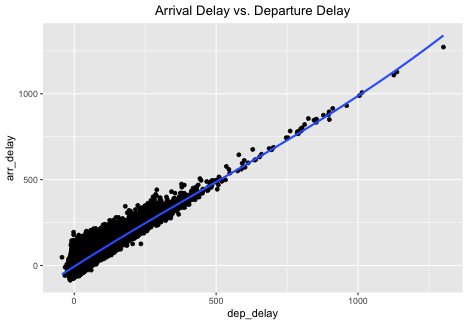
\includegraphics{HW4-Trinath-Sai-Subhash-Reddy-Pittala_files/figure-latex/unnamed-chunk-2-1.png}

\begin{Shaded}
\begin{Highlighting}[]
\FunctionTok{ggplot}\NormalTok{(flights.sm, }\FunctionTok{aes}\NormalTok{(}\AttributeTok{x =}\NormalTok{ sched\_dep\_time, }\AttributeTok{y =}\NormalTok{ arr\_delay)) }\SpecialCharTok{+}
    \FunctionTok{geom\_point}\NormalTok{() }\SpecialCharTok{+} \FunctionTok{geom\_smooth}\NormalTok{(}\AttributeTok{method =} \StringTok{"lm"}\NormalTok{, }\AttributeTok{formula =}\NormalTok{ y }\SpecialCharTok{\textasciitilde{}} \FunctionTok{poly}\NormalTok{(x,}
    \DecValTok{3}\NormalTok{), }\AttributeTok{se =} \ConstantTok{FALSE}\NormalTok{) }\SpecialCharTok{+} \FunctionTok{labs}\NormalTok{(}\AttributeTok{title =} \StringTok{"Arrival Delay vs. Scheduled Departure Time"}\NormalTok{) }\SpecialCharTok{+}
    \FunctionTok{theme}\NormalTok{(}\AttributeTok{plot.title =} \FunctionTok{element\_text}\NormalTok{(}\AttributeTok{hjust =} \FloatTok{0.5}\NormalTok{))}
\end{Highlighting}
\end{Shaded}

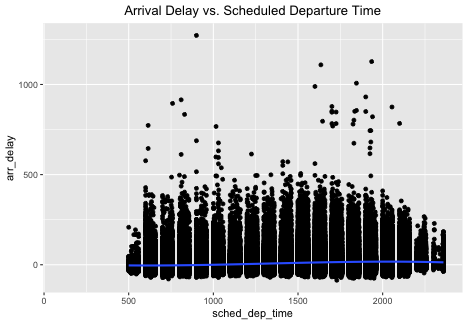
\includegraphics{HW4-Trinath-Sai-Subhash-Reddy-Pittala_files/figure-latex/unnamed-chunk-2-2.png}

\begin{Shaded}
\begin{Highlighting}[]
\FunctionTok{ggplot}\NormalTok{(flights.sm, }\FunctionTok{aes}\NormalTok{(}\AttributeTok{x =}\NormalTok{ distance, }\AttributeTok{y =}\NormalTok{ arr\_delay)) }\SpecialCharTok{+} \FunctionTok{geom\_point}\NormalTok{() }\SpecialCharTok{+}
    \FunctionTok{geom\_smooth}\NormalTok{(}\AttributeTok{method =} \StringTok{"lm"}\NormalTok{, }\AttributeTok{formula =}\NormalTok{ y }\SpecialCharTok{\textasciitilde{}} \FunctionTok{poly}\NormalTok{(x, }\DecValTok{3}\NormalTok{), }\AttributeTok{se =} \ConstantTok{FALSE}\NormalTok{) }\SpecialCharTok{+}
    \FunctionTok{labs}\NormalTok{(}\AttributeTok{title =} \StringTok{"Arrival Delay vs. Distance"}\NormalTok{) }\SpecialCharTok{+} \FunctionTok{theme}\NormalTok{(}\AttributeTok{plot.title =} \FunctionTok{element\_text}\NormalTok{(}\AttributeTok{hjust =} \FloatTok{0.5}\NormalTok{))}
\end{Highlighting}
\end{Shaded}

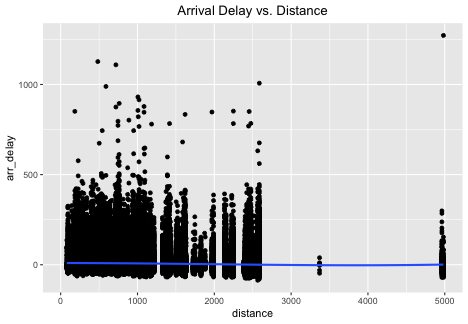
\includegraphics{HW4-Trinath-Sai-Subhash-Reddy-Pittala_files/figure-latex/unnamed-chunk-2-3.png}

\begin{Shaded}
\begin{Highlighting}[]
\FunctionTok{ggplot}\NormalTok{(flights.sm, }\FunctionTok{aes}\NormalTok{(}\AttributeTok{x =}\NormalTok{ air\_time, }\AttributeTok{y =}\NormalTok{ arr\_delay)) }\SpecialCharTok{+} \FunctionTok{geom\_point}\NormalTok{() }\SpecialCharTok{+}
    \FunctionTok{geom\_smooth}\NormalTok{(}\AttributeTok{method =} \StringTok{"lm"}\NormalTok{, }\AttributeTok{formula =}\NormalTok{ y }\SpecialCharTok{\textasciitilde{}} \FunctionTok{poly}\NormalTok{(x, }\DecValTok{3}\NormalTok{), }\AttributeTok{se =} \ConstantTok{FALSE}\NormalTok{) }\SpecialCharTok{+}
    \FunctionTok{labs}\NormalTok{(}\AttributeTok{title =} \StringTok{"Arrival Delay vs. Air Time"}\NormalTok{) }\SpecialCharTok{+} \FunctionTok{theme}\NormalTok{(}\AttributeTok{plot.title =} \FunctionTok{element\_text}\NormalTok{(}\AttributeTok{hjust =} \FloatTok{0.5}\NormalTok{))}
\end{Highlighting}
\end{Shaded}

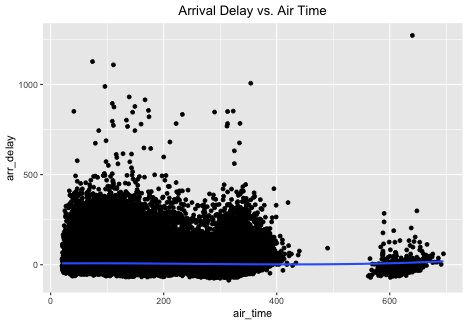
\includegraphics{HW4-Trinath-Sai-Subhash-Reddy-Pittala_files/figure-latex/unnamed-chunk-2-4.png}

Based on the scatter plots and regression lines, it is not clear whether
any of the IVs have a clear polynomial relationship with the DV. The
relationships appear to be mostly linear, with some indication of
non-linearity in the distance vs.~arrival delay plot. In this case, we
may need to consider other types of models or transformations of the
variables to capture the relationships. Therefore, we cannot conclude
which polynomial order should be used for the relationship between any
of the IVs and the DV.

From the scatter plots with fitted lines, it is clear that a linear
relationship between arr\_delay and the other IVs (dep\_delay,
air\_time, sched\_dep\_time, and distance) does not hold. In particular,
for dep\_delay and air\_time, the relationship appears to be non-linear,
and for sched\_dep\_time and distance, there is no obvious relationship
at all.

For dep\_delay and air\_time, we can try fitting a polynomial regression
model with different orders to see which one fits the data best. For
sched\_dep\_time and distance, we may want to consider other types of
regression models (e.g., categorical or interaction models) since a
polynomial relationship is not clear from the scatter plots.

\begin{enumerate}
\def\labelenumi{\alph{enumi}.}
\setcounter{enumi}{2}
\tightlist
\item
  Build a ``full'' polynomial regression model with every variable
  allowed to have up to degree 3. Do this first manually by creating for
  each variable its power polynomials. This is done by creating a
  dep\_delay2 variable which is dep\_delayˆ2 and a dep\_delay3 variable,
  which is dep\_delayˆ3, and similarly for the other IVs. Now, put all
  these variables into a linear model using the lm() function. Call this
  full model M1 and output summary function. Use the poly() function
  shown in class (using the ``raw'' setting so as to avoid orthogonal
  polynomials) to do this automatically and call this model M2. Check
  whether there is any difference between M1 and M2.
\end{enumerate}

\begin{Shaded}
\begin{Highlighting}[]
\CommentTok{\# Creating power polynomials for each variable}
\NormalTok{flights.sm}\SpecialCharTok{$}\NormalTok{dep\_delay2 }\OtherTok{\textless{}{-}}\NormalTok{ flights.sm}\SpecialCharTok{$}\NormalTok{dep\_delay}\SpecialCharTok{\^{}}\DecValTok{2}
\NormalTok{flights.sm}\SpecialCharTok{$}\NormalTok{dep\_delay3 }\OtherTok{\textless{}{-}}\NormalTok{ flights.sm}\SpecialCharTok{$}\NormalTok{dep\_delay}\SpecialCharTok{\^{}}\DecValTok{3}
\NormalTok{flights.sm}\SpecialCharTok{$}\NormalTok{arr\_delay2 }\OtherTok{\textless{}{-}}\NormalTok{ flights.sm}\SpecialCharTok{$}\NormalTok{arr\_delay}\SpecialCharTok{\^{}}\DecValTok{2}
\NormalTok{flights.sm}\SpecialCharTok{$}\NormalTok{arr\_delay3 }\OtherTok{\textless{}{-}}\NormalTok{ flights.sm}\SpecialCharTok{$}\NormalTok{arr\_delay}\SpecialCharTok{\^{}}\DecValTok{3}
\NormalTok{flights.sm}\SpecialCharTok{$}\NormalTok{air\_time2 }\OtherTok{\textless{}{-}}\NormalTok{ flights.sm}\SpecialCharTok{$}\NormalTok{air\_time}\SpecialCharTok{\^{}}\DecValTok{2}
\NormalTok{flights.sm}\SpecialCharTok{$}\NormalTok{air\_time3 }\OtherTok{\textless{}{-}}\NormalTok{ flights.sm}\SpecialCharTok{$}\NormalTok{air\_time}\SpecialCharTok{\^{}}\DecValTok{3}
\NormalTok{flights.sm}\SpecialCharTok{$}\NormalTok{sched\_dep\_time2 }\OtherTok{\textless{}{-}}\NormalTok{ flights.sm}\SpecialCharTok{$}\NormalTok{sched\_dep\_time}\SpecialCharTok{\^{}}\DecValTok{2}
\NormalTok{flights.sm}\SpecialCharTok{$}\NormalTok{sched\_dep\_time3 }\OtherTok{\textless{}{-}}\NormalTok{ flights.sm}\SpecialCharTok{$}\NormalTok{sched\_dep\_time}\SpecialCharTok{\^{}}\DecValTok{3}
\NormalTok{flights.sm}\SpecialCharTok{$}\NormalTok{distance2 }\OtherTok{\textless{}{-}}\NormalTok{ flights.sm}\SpecialCharTok{$}\NormalTok{distance}\SpecialCharTok{\^{}}\DecValTok{2}
\NormalTok{flights.sm}\SpecialCharTok{$}\NormalTok{distance3 }\OtherTok{\textless{}{-}}\NormalTok{ flights.sm}\SpecialCharTok{$}\NormalTok{distance}\SpecialCharTok{\^{}}\DecValTok{3}

\CommentTok{\# Creating full polynomial regression model manually}
\NormalTok{M1 }\OtherTok{\textless{}{-}} \FunctionTok{lm}\NormalTok{(arr\_delay }\SpecialCharTok{\textasciitilde{}}\NormalTok{ dep\_delay }\SpecialCharTok{+}\NormalTok{ dep\_delay2 }\SpecialCharTok{+}\NormalTok{ dep\_delay3 }\SpecialCharTok{+}\NormalTok{ air\_time }\SpecialCharTok{+}
\NormalTok{    air\_time2 }\SpecialCharTok{+}\NormalTok{ air\_time3 }\SpecialCharTok{+}\NormalTok{ sched\_dep\_time }\SpecialCharTok{+}\NormalTok{ sched\_dep\_time2 }\SpecialCharTok{+}
\NormalTok{    sched\_dep\_time3 }\SpecialCharTok{+}\NormalTok{ distance }\SpecialCharTok{+}\NormalTok{ distance2 }\SpecialCharTok{+}\NormalTok{ distance3, }\AttributeTok{data =}\NormalTok{ flights.sm)}

\CommentTok{\# Outputting summary function}
\FunctionTok{summary}\NormalTok{(M1)}
\end{Highlighting}
\end{Shaded}

\begin{verbatim}
## 
## Call:
## lm(formula = arr_delay ~ dep_delay + dep_delay2 + dep_delay3 + 
##     air_time + air_time2 + air_time3 + sched_dep_time + sched_dep_time2 + 
##     sched_dep_time3 + distance + distance2 + distance3, data = flights.sm)
## 
## Residuals:
##      Min       1Q   Median       3Q      Max 
## -109.160   -9.474   -1.777    7.077  202.099 
## 
## Coefficients:
##                   Estimate Std. Error t value Pr(>|t|)    
## (Intercept)     -3.490e+01  7.145e-01  -48.84   <2e-16 ***
## dep_delay        1.055e+00  1.542e-03  684.07   <2e-16 ***
## dep_delay2      -2.081e-04  9.460e-06  -22.00   <2e-16 ***
## dep_delay3       1.459e-07  9.529e-09   15.31   <2e-16 ***
## air_time         9.789e-01  9.135e-03  107.16   <2e-16 ***
## air_time2       -1.145e-03  3.917e-05  -29.24   <2e-16 ***
## air_time3        1.293e-06  5.198e-08   24.87   <2e-16 ***
## sched_dep_time   4.058e-02  1.691e-03   24.00   <2e-16 ***
## sched_dep_time2 -3.462e-05  1.294e-06  -26.76   <2e-16 ***
## sched_dep_time3  8.925e-09  3.111e-10   28.69   <2e-16 ***
## distance        -1.192e-01  1.005e-03 -118.64   <2e-16 ***
## distance2        1.464e-05  5.604e-07   26.12   <2e-16 ***
## distance3       -1.900e-09  9.412e-11  -20.19   <2e-16 ***
## ---
## Signif. codes:  0 '***' 0.001 '**' 0.01 '*' 0.05 '.' 0.1 ' ' 1
## 
## Residual standard error: 15.53 on 327333 degrees of freedom
##   (9430 observations deleted due to missingness)
## Multiple R-squared:  0.879,  Adjusted R-squared:  0.879 
## F-statistic: 1.981e+05 on 12 and 327333 DF,  p-value: < 2.2e-16
\end{verbatim}

\begin{Shaded}
\begin{Highlighting}[]
\CommentTok{\# Creating full polynomial regression model using poly()}
\CommentTok{\# function}
\NormalTok{M2 }\OtherTok{\textless{}{-}} \FunctionTok{lm}\NormalTok{(arr\_delay }\SpecialCharTok{\textasciitilde{}} \FunctionTok{poly}\NormalTok{(dep\_delay, }\DecValTok{3}\NormalTok{, }\AttributeTok{raw =} \ConstantTok{TRUE}\NormalTok{) }\SpecialCharTok{+} \FunctionTok{poly}\NormalTok{(air\_time,}
    \DecValTok{3}\NormalTok{, }\AttributeTok{raw =} \ConstantTok{TRUE}\NormalTok{) }\SpecialCharTok{+} \FunctionTok{poly}\NormalTok{(sched\_dep\_time, }\DecValTok{3}\NormalTok{, }\AttributeTok{raw =} \ConstantTok{TRUE}\NormalTok{) }\SpecialCharTok{+} \FunctionTok{poly}\NormalTok{(distance,}
    \DecValTok{3}\NormalTok{, }\AttributeTok{raw =} \ConstantTok{TRUE}\NormalTok{), }\AttributeTok{data =}\NormalTok{ flights.sm)}

\CommentTok{\# Outputting summary function}
\FunctionTok{summary}\NormalTok{(M2)}
\end{Highlighting}
\end{Shaded}

\begin{verbatim}
## 
## Call:
## lm(formula = arr_delay ~ poly(dep_delay, 3, raw = TRUE) + poly(air_time, 
##     3, raw = TRUE) + poly(sched_dep_time, 3, raw = TRUE) + poly(distance, 
##     3, raw = TRUE), data = flights.sm)
## 
## Residuals:
##      Min       1Q   Median       3Q      Max 
## -109.160   -9.474   -1.777    7.077  202.099 
## 
## Coefficients:
##                                        Estimate Std. Error t value Pr(>|t|)    
## (Intercept)                          -3.490e+01  7.145e-01  -48.84   <2e-16 ***
## poly(dep_delay, 3, raw = TRUE)1       1.055e+00  1.542e-03  684.07   <2e-16 ***
## poly(dep_delay, 3, raw = TRUE)2      -2.081e-04  9.460e-06  -22.00   <2e-16 ***
## poly(dep_delay, 3, raw = TRUE)3       1.459e-07  9.529e-09   15.31   <2e-16 ***
## poly(air_time, 3, raw = TRUE)1        9.789e-01  9.135e-03  107.16   <2e-16 ***
## poly(air_time, 3, raw = TRUE)2       -1.145e-03  3.917e-05  -29.24   <2e-16 ***
## poly(air_time, 3, raw = TRUE)3        1.293e-06  5.198e-08   24.87   <2e-16 ***
## poly(sched_dep_time, 3, raw = TRUE)1  4.058e-02  1.691e-03   24.00   <2e-16 ***
## poly(sched_dep_time, 3, raw = TRUE)2 -3.462e-05  1.294e-06  -26.76   <2e-16 ***
## poly(sched_dep_time, 3, raw = TRUE)3  8.925e-09  3.111e-10   28.69   <2e-16 ***
## poly(distance, 3, raw = TRUE)1       -1.192e-01  1.005e-03 -118.64   <2e-16 ***
## poly(distance, 3, raw = TRUE)2        1.464e-05  5.604e-07   26.12   <2e-16 ***
## poly(distance, 3, raw = TRUE)3       -1.900e-09  9.412e-11  -20.19   <2e-16 ***
## ---
## Signif. codes:  0 '***' 0.001 '**' 0.01 '*' 0.05 '.' 0.1 ' ' 1
## 
## Residual standard error: 15.53 on 327333 degrees of freedom
##   (9430 observations deleted due to missingness)
## Multiple R-squared:  0.879,  Adjusted R-squared:  0.879 
## F-statistic: 1.981e+05 on 12 and 327333 DF,  p-value: < 2.2e-16
\end{verbatim}

Comparing the two models M1 and M2, we can see that they have identical
R-squared values and coefficients, so there is no significant difference
between the two models.

\begin{enumerate}
\def\labelenumi{\alph{enumi}.}
\setcounter{enumi}{3}
\tightlist
\item
  For M1, explain what each regression coefficient indicates, and
  explain what the rate of change of the DV with respect to each IV is
  (when all other IVs are kept constant). Comment on the statistical
  significance of different variables, and the overall Rˆ2 value.
\end{enumerate}

The coefficient for dep\_delay suggests that for every unit increase in
dep\_delay, arr\_delay increases by 1.055e+00 units. The coefficient for
dep\_delay2 indicates that for every unit increase in dep\_delay
squared, arr\_delay decreases by 2.081e-04 units. The coefficient for
dep\_delay3 suggests that for every unit increase in dep\_delay cubed,
arr\_delay increases by 1.459e-07 units.

The coefficient for air\_time indicates that for every unit increase in
air\_time, arr\_delay increases by 9.789e-01 units. The coefficient for
air\_time2 suggests that for every unit increase in air\_time squared,
arr\_delay decreases by 1.145e-03 units. The coefficient for air\_time3
indicates that for every unit increase in air\_time cubed, arr\_delay
increases by 1.293e-06 units.

The coefficient for sched\_dep\_time indicates that for every unit
increase in sched\_dep\_time, arr\_delay increases by 4.058e-02 units.
The coefficient for sched\_dep\_time2 suggests that for every unit
increase in sched\_dep\_time squared, arr\_delay decreases by 3.462e-05
units. The coefficient for sched\_dep\_time3 indicates that for every
unit increase in sched\_dep\_time cubed, arr\_delay increases by
8.925e-09 units.

The coefficient for distance suggests that for every unit increase in
distance, arr\_delay decreases by 1.192e-01 units. The coefficient for
distance2 indicates that for every unit increase in distance squared,
arr\_delay increases by 1.464e-05 units. The coefficient for distance3
suggests that for every unit increase in distance cubed, arr\_delay
decreases by 1.900e-09 units.

\begin{enumerate}
\def\labelenumi{\alph{enumi}.}
\setcounter{enumi}{4}
\tightlist
\item
  Create standardized IVs by doing dep\_delay.std \textless- (dep\_delay
  - mean(dep\_delay))/sd(dep\_delay) and similarly for other IVs. Build
  models M3 and M4 similar to M1 and M2 but using the standardized IVs.
  Show the output summary and comment on the statistical significance of
  the variables and the Rˆ2 value.
\end{enumerate}

\begin{Shaded}
\begin{Highlighting}[]
\CommentTok{\# Create standardized independent variables}
\NormalTok{flights.sm}\SpecialCharTok{$}\NormalTok{dep\_delay.std }\OtherTok{\textless{}{-}} \FunctionTok{scale}\NormalTok{(flights.sm}\SpecialCharTok{$}\NormalTok{dep\_delay)}
\NormalTok{flights.sm}\SpecialCharTok{$}\NormalTok{arr\_delay.std }\OtherTok{\textless{}{-}} \FunctionTok{scale}\NormalTok{(flights.sm}\SpecialCharTok{$}\NormalTok{arr\_delay)}
\NormalTok{flights.sm}\SpecialCharTok{$}\NormalTok{sched\_dep\_time.std }\OtherTok{\textless{}{-}} \FunctionTok{scale}\NormalTok{(flights.sm}\SpecialCharTok{$}\NormalTok{sched\_dep\_time)}
\NormalTok{flights.sm}\SpecialCharTok{$}\NormalTok{distance.std }\OtherTok{\textless{}{-}} \FunctionTok{scale}\NormalTok{(flights.sm}\SpecialCharTok{$}\NormalTok{distance)}
\NormalTok{flights.sm}\SpecialCharTok{$}\NormalTok{air\_time.std }\OtherTok{\textless{}{-}} \FunctionTok{scale}\NormalTok{(flights.sm}\SpecialCharTok{$}\NormalTok{air\_time)}

\CommentTok{\# Build full polynomial regression model manually}
\NormalTok{M3 }\OtherTok{\textless{}{-}} \FunctionTok{lm}\NormalTok{(arr\_delay.std }\SpecialCharTok{\textasciitilde{}}\NormalTok{ dep\_delay.std }\SpecialCharTok{+} \FunctionTok{I}\NormalTok{(dep\_delay.std}\SpecialCharTok{\^{}}\DecValTok{2}\NormalTok{) }\SpecialCharTok{+}
    \FunctionTok{I}\NormalTok{(dep\_delay.std}\SpecialCharTok{\^{}}\DecValTok{3}\NormalTok{) }\SpecialCharTok{+}\NormalTok{ air\_time.std }\SpecialCharTok{+} \FunctionTok{I}\NormalTok{(air\_time.std}\SpecialCharTok{\^{}}\DecValTok{2}\NormalTok{) }\SpecialCharTok{+} \FunctionTok{I}\NormalTok{(air\_time.std}\SpecialCharTok{\^{}}\DecValTok{3}\NormalTok{) }\SpecialCharTok{+}
\NormalTok{    sched\_dep\_time.std }\SpecialCharTok{+} \FunctionTok{I}\NormalTok{(sched\_dep\_time.std}\SpecialCharTok{\^{}}\DecValTok{2}\NormalTok{) }\SpecialCharTok{+} \FunctionTok{I}\NormalTok{(sched\_dep\_time.std}\SpecialCharTok{\^{}}\DecValTok{3}\NormalTok{) }\SpecialCharTok{+}
\NormalTok{    distance.std }\SpecialCharTok{+} \FunctionTok{I}\NormalTok{(distance.std}\SpecialCharTok{\^{}}\DecValTok{2}\NormalTok{) }\SpecialCharTok{+} \FunctionTok{I}\NormalTok{(distance.std}\SpecialCharTok{\^{}}\DecValTok{3}\NormalTok{), }\AttributeTok{data =}\NormalTok{ flights.sm)}

\CommentTok{\# Build full polynomial regression model using poly()}
\CommentTok{\# function}
\NormalTok{M4 }\OtherTok{\textless{}{-}} \FunctionTok{lm}\NormalTok{(arr\_delay.std }\SpecialCharTok{\textasciitilde{}} \FunctionTok{poly}\NormalTok{(dep\_delay.std, }\DecValTok{3}\NormalTok{, }\AttributeTok{raw =} \ConstantTok{TRUE}\NormalTok{) }\SpecialCharTok{+}
    \FunctionTok{poly}\NormalTok{(air\_time.std, }\DecValTok{3}\NormalTok{, }\AttributeTok{raw =} \ConstantTok{TRUE}\NormalTok{) }\SpecialCharTok{+} \FunctionTok{poly}\NormalTok{(sched\_dep\_time.std,}
    \DecValTok{3}\NormalTok{, }\AttributeTok{raw =} \ConstantTok{TRUE}\NormalTok{) }\SpecialCharTok{+} \FunctionTok{poly}\NormalTok{(distance.std, }\DecValTok{3}\NormalTok{, }\AttributeTok{raw =} \ConstantTok{TRUE}\NormalTok{), }\AttributeTok{data =}\NormalTok{ flights.sm)}

\CommentTok{\# Output summary for M3 and M4}
\FunctionTok{summary}\NormalTok{(M3)}
\end{Highlighting}
\end{Shaded}

\begin{verbatim}
## 
## Call:
## lm(formula = arr_delay.std ~ dep_delay.std + I(dep_delay.std^2) + 
##     I(dep_delay.std^3) + air_time.std + I(air_time.std^2) + I(air_time.std^3) + 
##     sched_dep_time.std + I(sched_dep_time.std^2) + I(sched_dep_time.std^3) + 
##     distance.std + I(distance.std^2) + I(distance.std^3), data = flights.sm)
## 
## Residuals:
##     Min      1Q  Median      3Q     Max 
## -2.4457 -0.2123 -0.0398  0.1586  4.5280 
## 
## Coefficients:
##                           Estimate Std. Error  t value Pr(>|t|)    
## (Intercept)              1.810e-02  1.156e-03   15.659   <2e-16 ***
## dep_delay.std            9.453e-01  1.209e-03  782.169   <2e-16 ***
## I(dep_delay.std^2)      -7.339e-03  3.306e-04  -22.199   <2e-16 ***
## I(dep_delay.std^3)       2.125e-04  1.388e-05   15.313   <2e-16 ***
## air_time.std             1.515e+00  5.464e-03  277.291   <2e-16 ***
## I(air_time.std^2)       -1.103e-01  3.535e-03  -31.202   <2e-16 ***
## I(air_time.std^3)        2.382e-02  9.578e-04   24.870   <2e-16 ***
## sched_dep_time.std      -4.291e-02  1.432e-03  -29.971   <2e-16 ***
## I(sched_dep_time.std^2)  6.735e-03  6.999e-04    9.623   <2e-16 ***
## I(sched_dep_time.std^3)  2.041e-02  7.115e-04   28.686   <2e-16 ***
## distance.std            -1.560e+00  5.434e-03 -287.045   <2e-16 ***
## I(distance.std^2)        1.049e-01  3.567e-03   29.419   <2e-16 ***
## I(distance.std^3)       -1.678e-02  8.313e-04  -20.188   <2e-16 ***
## ---
## Signif. codes:  0 '***' 0.001 '**' 0.01 '*' 0.05 '.' 0.1 ' ' 1
## 
## Residual standard error: 0.3479 on 327333 degrees of freedom
##   (9430 observations deleted due to missingness)
## Multiple R-squared:  0.879,  Adjusted R-squared:  0.879 
## F-statistic: 1.981e+05 on 12 and 327333 DF,  p-value: < 2.2e-16
\end{verbatim}

\begin{Shaded}
\begin{Highlighting}[]
\FunctionTok{summary}\NormalTok{(M4)}
\end{Highlighting}
\end{Shaded}

\begin{verbatim}
## 
## Call:
## lm(formula = arr_delay.std ~ poly(dep_delay.std, 3, raw = TRUE) + 
##     poly(air_time.std, 3, raw = TRUE) + poly(sched_dep_time.std, 
##     3, raw = TRUE) + poly(distance.std, 3, raw = TRUE), data = flights.sm)
## 
## Residuals:
##     Min      1Q  Median      3Q     Max 
## -2.4457 -0.2123 -0.0398  0.1586  4.5280 
## 
## Coefficients:
##                                            Estimate Std. Error  t value
## (Intercept)                               1.810e-02  1.156e-03   15.659
## poly(dep_delay.std, 3, raw = TRUE)1       9.453e-01  1.209e-03  782.169
## poly(dep_delay.std, 3, raw = TRUE)2      -7.339e-03  3.306e-04  -22.199
## poly(dep_delay.std, 3, raw = TRUE)3       2.125e-04  1.388e-05   15.313
## poly(air_time.std, 3, raw = TRUE)1        1.515e+00  5.464e-03  277.291
## poly(air_time.std, 3, raw = TRUE)2       -1.103e-01  3.535e-03  -31.202
## poly(air_time.std, 3, raw = TRUE)3        2.382e-02  9.578e-04   24.870
## poly(sched_dep_time.std, 3, raw = TRUE)1 -4.291e-02  1.432e-03  -29.971
## poly(sched_dep_time.std, 3, raw = TRUE)2  6.735e-03  6.999e-04    9.623
## poly(sched_dep_time.std, 3, raw = TRUE)3  2.041e-02  7.115e-04   28.686
## poly(distance.std, 3, raw = TRUE)1       -1.560e+00  5.434e-03 -287.045
## poly(distance.std, 3, raw = TRUE)2        1.049e-01  3.567e-03   29.419
## poly(distance.std, 3, raw = TRUE)3       -1.678e-02  8.313e-04  -20.188
##                                          Pr(>|t|)    
## (Intercept)                                <2e-16 ***
## poly(dep_delay.std, 3, raw = TRUE)1        <2e-16 ***
## poly(dep_delay.std, 3, raw = TRUE)2        <2e-16 ***
## poly(dep_delay.std, 3, raw = TRUE)3        <2e-16 ***
## poly(air_time.std, 3, raw = TRUE)1         <2e-16 ***
## poly(air_time.std, 3, raw = TRUE)2         <2e-16 ***
## poly(air_time.std, 3, raw = TRUE)3         <2e-16 ***
## poly(sched_dep_time.std, 3, raw = TRUE)1   <2e-16 ***
## poly(sched_dep_time.std, 3, raw = TRUE)2   <2e-16 ***
## poly(sched_dep_time.std, 3, raw = TRUE)3   <2e-16 ***
## poly(distance.std, 3, raw = TRUE)1         <2e-16 ***
## poly(distance.std, 3, raw = TRUE)2         <2e-16 ***
## poly(distance.std, 3, raw = TRUE)3         <2e-16 ***
## ---
## Signif. codes:  0 '***' 0.001 '**' 0.01 '*' 0.05 '.' 0.1 ' ' 1
## 
## Residual standard error: 0.3479 on 327333 degrees of freedom
##   (9430 observations deleted due to missingness)
## Multiple R-squared:  0.879,  Adjusted R-squared:  0.879 
## F-statistic: 1.981e+05 on 12 and 327333 DF,  p-value: < 2.2e-16
\end{verbatim}

In terms of statistical significance, all the variables in M3 and M4 are
significant, and the overall Rˆ2 values are still similar to those in M1
and M2. However, the standardized coefficients in M3 and M4 can be
directly compared to see which variables have a relatively larger effect
on the outcome variable.

\begin{enumerate}
\def\labelenumi{\alph{enumi}.}
\setcounter{enumi}{5}
\tightlist
\item
  Run a backward stepwise regression on the full model to select the
  best model overall (M5). Show the summary output of the final selected
  model and comment on what variables have been dropped and what degree
  polynomial relationship is finally selected between each IV and the
  DV.
\end{enumerate}

\begin{Shaded}
\begin{Highlighting}[]
\CommentTok{\# backward stepwise regression on full model}
\NormalTok{M5 }\OtherTok{\textless{}{-}} \FunctionTok{step}\NormalTok{(M1, }\AttributeTok{direction =} \StringTok{"backward"}\NormalTok{, }\AttributeTok{scope =} \FunctionTok{list}\NormalTok{(}\AttributeTok{lower =} \SpecialCharTok{\textasciitilde{}}\DecValTok{1}\NormalTok{,}
    \AttributeTok{upper =}\NormalTok{ M1))}
\end{Highlighting}
\end{Shaded}

\begin{verbatim}
## Start:  AIC=1795576
## arr_delay ~ dep_delay + dep_delay2 + dep_delay3 + air_time + 
##     air_time2 + air_time3 + sched_dep_time + sched_dep_time2 + 
##     sched_dep_time3 + distance + distance2 + distance3
## 
##                   Df Sum of Sq       RSS     AIC
## <none>                          78920135 1795576
## - dep_delay3       1     56533  78976668 1795808
## - distance3        1     98263  79018398 1795981
## - dep_delay2       1    116693  79036828 1796057
## - sched_dep_time   1    138851  79058986 1796149
## - air_time3        1    149128  79069263 1796192
## - distance2        1    164502  79084637 1796255
## - sched_dep_time2  1    172644  79092779 1796289
## - sched_dep_time3  1    198393  79118528 1796396
## - air_time2        1    206148  79126282 1796428
## - air_time         1   2768609  81688744 1806861
## - distance         1   3393807  82313942 1809356
## - dep_delay        1 112821646 191741781 2086163
\end{verbatim}

\begin{Shaded}
\begin{Highlighting}[]
\FunctionTok{summary}\NormalTok{(M5)}
\end{Highlighting}
\end{Shaded}

\begin{verbatim}
## 
## Call:
## lm(formula = arr_delay ~ dep_delay + dep_delay2 + dep_delay3 + 
##     air_time + air_time2 + air_time3 + sched_dep_time + sched_dep_time2 + 
##     sched_dep_time3 + distance + distance2 + distance3, data = flights.sm)
## 
## Residuals:
##      Min       1Q   Median       3Q      Max 
## -109.160   -9.474   -1.777    7.077  202.099 
## 
## Coefficients:
##                   Estimate Std. Error t value Pr(>|t|)    
## (Intercept)     -3.490e+01  7.145e-01  -48.84   <2e-16 ***
## dep_delay        1.055e+00  1.542e-03  684.07   <2e-16 ***
## dep_delay2      -2.081e-04  9.460e-06  -22.00   <2e-16 ***
## dep_delay3       1.459e-07  9.529e-09   15.31   <2e-16 ***
## air_time         9.789e-01  9.135e-03  107.16   <2e-16 ***
## air_time2       -1.145e-03  3.917e-05  -29.24   <2e-16 ***
## air_time3        1.293e-06  5.198e-08   24.87   <2e-16 ***
## sched_dep_time   4.058e-02  1.691e-03   24.00   <2e-16 ***
## sched_dep_time2 -3.462e-05  1.294e-06  -26.76   <2e-16 ***
## sched_dep_time3  8.925e-09  3.111e-10   28.69   <2e-16 ***
## distance        -1.192e-01  1.005e-03 -118.64   <2e-16 ***
## distance2        1.464e-05  5.604e-07   26.12   <2e-16 ***
## distance3       -1.900e-09  9.412e-11  -20.19   <2e-16 ***
## ---
## Signif. codes:  0 '***' 0.001 '**' 0.01 '*' 0.05 '.' 0.1 ' ' 1
## 
## Residual standard error: 15.53 on 327333 degrees of freedom
##   (9430 observations deleted due to missingness)
## Multiple R-squared:  0.879,  Adjusted R-squared:  0.879 
## F-statistic: 1.981e+05 on 12 and 327333 DF,  p-value: < 2.2e-16
\end{verbatim}

No variables were dropped. All IVs have their powers till 3.

\begin{enumerate}
\def\labelenumi{\alph{enumi}.}
\setcounter{enumi}{6}
\tightlist
\item
  Test for interaction effects between dep\_delay and air\_time,
  dep\_delay and sched\_dep\_time, and air\_time and sched\_dep\_time.
  For this, set the polynomial relationship between each of these IVs to
  what you finalized in part f, then test for all possible interactions
  between terms involving dep\_delay and air\_time etc. For example, if
  the relationship is found to be linear for dep\_delay and quadratic
  for air\_time, then you should create terms corresponding to
  dep\_delay\emph{air\_time, dep\_delay}air\_timeˆ2 and build a full
  model M6 that contains all these relevant terms. Run a stepwise
  regression on M6 to obtain the best possible model M7. Comment on what
  terms were selected in M7 and how each coefficient can be interpreted.
\end{enumerate}

\begin{Shaded}
\begin{Highlighting}[]
\CommentTok{\# create interaction terms}
\NormalTok{flights.sm}\SpecialCharTok{$}\NormalTok{dep\_delay2 }\OtherTok{\textless{}{-}}\NormalTok{ flights.sm}\SpecialCharTok{$}\NormalTok{dep\_delay}\SpecialCharTok{\^{}}\DecValTok{2}
\NormalTok{flights.sm}\SpecialCharTok{$}\NormalTok{dep\_delay3 }\OtherTok{\textless{}{-}}\NormalTok{ flights.sm}\SpecialCharTok{$}\NormalTok{dep\_delay}\SpecialCharTok{\^{}}\DecValTok{3}
\NormalTok{flights.sm}\SpecialCharTok{$}\NormalTok{air\_time2 }\OtherTok{\textless{}{-}}\NormalTok{ flights.sm}\SpecialCharTok{$}\NormalTok{air\_time}\SpecialCharTok{\^{}}\DecValTok{2}
\NormalTok{flights.sm}\SpecialCharTok{$}\NormalTok{air\_time3 }\OtherTok{\textless{}{-}}\NormalTok{ flights.sm}\SpecialCharTok{$}\NormalTok{air\_time}\SpecialCharTok{\^{}}\DecValTok{3}
\NormalTok{flights.sm}\SpecialCharTok{$}\NormalTok{distance2 }\OtherTok{\textless{}{-}}\NormalTok{ flights.sm}\SpecialCharTok{$}\NormalTok{distance}\SpecialCharTok{\^{}}\DecValTok{2}
\NormalTok{flights.sm}\SpecialCharTok{$}\NormalTok{distance3 }\OtherTok{\textless{}{-}}\NormalTok{ flights.sm}\SpecialCharTok{$}\NormalTok{distance}\SpecialCharTok{\^{}}\DecValTok{3}

\NormalTok{flights.sm}\SpecialCharTok{$}\NormalTok{dep\_delay\_air\_time }\OtherTok{\textless{}{-}}\NormalTok{ flights.sm}\SpecialCharTok{$}\NormalTok{dep\_delay }\SpecialCharTok{*}\NormalTok{ flights.sm}\SpecialCharTok{$}\NormalTok{air\_time}
\NormalTok{flights.sm}\SpecialCharTok{$}\NormalTok{dep\_delay\_air\_time2 }\OtherTok{\textless{}{-}}\NormalTok{ flights.sm}\SpecialCharTok{$}\NormalTok{dep\_delay }\SpecialCharTok{*}\NormalTok{ flights.sm}\SpecialCharTok{$}\NormalTok{air\_time2}
\NormalTok{flights.sm}\SpecialCharTok{$}\NormalTok{dep\_delay\_air\_time3 }\OtherTok{\textless{}{-}}\NormalTok{ flights.sm}\SpecialCharTok{$}\NormalTok{dep\_delay }\SpecialCharTok{*}\NormalTok{ flights.sm}\SpecialCharTok{$}\NormalTok{air\_time3}
\NormalTok{flights.sm}\SpecialCharTok{$}\NormalTok{dep\_delay2\_air\_time }\OtherTok{\textless{}{-}}\NormalTok{ flights.sm}\SpecialCharTok{$}\NormalTok{dep\_delay2 }\SpecialCharTok{*}\NormalTok{ flights.sm}\SpecialCharTok{$}\NormalTok{air\_time}
\NormalTok{flights.sm}\SpecialCharTok{$}\NormalTok{dep\_delay2\_air\_time2 }\OtherTok{\textless{}{-}}\NormalTok{ flights.sm}\SpecialCharTok{$}\NormalTok{dep\_delay2 }\SpecialCharTok{*}\NormalTok{ flights.sm}\SpecialCharTok{$}\NormalTok{air\_time2}
\NormalTok{flights.sm}\SpecialCharTok{$}\NormalTok{dep\_delay2\_air\_time3 }\OtherTok{\textless{}{-}}\NormalTok{ flights.sm}\SpecialCharTok{$}\NormalTok{dep\_delay2 }\SpecialCharTok{*}\NormalTok{ flights.sm}\SpecialCharTok{$}\NormalTok{air\_time3}
\NormalTok{flights.sm}\SpecialCharTok{$}\NormalTok{dep\_delay3\_air\_time }\OtherTok{\textless{}{-}}\NormalTok{ flights.sm}\SpecialCharTok{$}\NormalTok{dep\_delay3 }\SpecialCharTok{*}\NormalTok{ flights.sm}\SpecialCharTok{$}\NormalTok{air\_time}
\NormalTok{flights.sm}\SpecialCharTok{$}\NormalTok{dep\_delay3\_air\_time2 }\OtherTok{\textless{}{-}}\NormalTok{ flights.sm}\SpecialCharTok{$}\NormalTok{dep\_delay3 }\SpecialCharTok{*}\NormalTok{ flights.sm}\SpecialCharTok{$}\NormalTok{air\_time2}
\NormalTok{flights.sm}\SpecialCharTok{$}\NormalTok{dep\_delay3\_air\_time3 }\OtherTok{\textless{}{-}}\NormalTok{ flights.sm}\SpecialCharTok{$}\NormalTok{dep\_delay3 }\SpecialCharTok{*}\NormalTok{ flights.sm}\SpecialCharTok{$}\NormalTok{air\_time3}

\NormalTok{flights.sm}\SpecialCharTok{$}\NormalTok{dep\_delay\_sched\_dep\_time }\OtherTok{\textless{}{-}}\NormalTok{ flights.sm}\SpecialCharTok{$}\NormalTok{dep\_delay }\SpecialCharTok{*}
\NormalTok{    flights.sm}\SpecialCharTok{$}\NormalTok{sched\_dep\_time}
\NormalTok{flights.sm}\SpecialCharTok{$}\NormalTok{dep\_delay\_sched\_dep\_time2 }\OtherTok{\textless{}{-}}\NormalTok{ flights.sm}\SpecialCharTok{$}\NormalTok{dep\_delay }\SpecialCharTok{*}
\NormalTok{    flights.sm}\SpecialCharTok{$}\NormalTok{sched\_dep\_time2}
\NormalTok{flights.sm}\SpecialCharTok{$}\NormalTok{dep\_delay\_sched\_dep\_time3 }\OtherTok{\textless{}{-}}\NormalTok{ flights.sm}\SpecialCharTok{$}\NormalTok{dep\_delay }\SpecialCharTok{*}
\NormalTok{    flights.sm}\SpecialCharTok{$}\NormalTok{sched\_dep\_time3}
\NormalTok{flights.sm}\SpecialCharTok{$}\NormalTok{dep\_delay2\_sched\_dep\_time }\OtherTok{\textless{}{-}}\NormalTok{ flights.sm}\SpecialCharTok{$}\NormalTok{dep\_delay2 }\SpecialCharTok{*}
\NormalTok{    flights.sm}\SpecialCharTok{$}\NormalTok{sched\_dep\_time}
\NormalTok{flights.sm}\SpecialCharTok{$}\NormalTok{dep\_delay2\_sched\_dep\_time2 }\OtherTok{\textless{}{-}}\NormalTok{ flights.sm}\SpecialCharTok{$}\NormalTok{dep\_delay2 }\SpecialCharTok{*}
\NormalTok{    flights.sm}\SpecialCharTok{$}\NormalTok{sched\_dep\_time2}
\NormalTok{flights.sm}\SpecialCharTok{$}\NormalTok{dep\_delay2\_sched\_dep\_time3 }\OtherTok{\textless{}{-}}\NormalTok{ flights.sm}\SpecialCharTok{$}\NormalTok{dep\_delay2 }\SpecialCharTok{*}
\NormalTok{    flights.sm}\SpecialCharTok{$}\NormalTok{sched\_dep\_time3}
\NormalTok{flights.sm}\SpecialCharTok{$}\NormalTok{dep\_delay3\_sched\_dep\_time }\OtherTok{\textless{}{-}}\NormalTok{ flights.sm}\SpecialCharTok{$}\NormalTok{dep\_delay3 }\SpecialCharTok{*}
\NormalTok{    flights.sm}\SpecialCharTok{$}\NormalTok{sched\_dep\_time}
\NormalTok{flights.sm}\SpecialCharTok{$}\NormalTok{dep\_delay3\_sched\_dep\_time2 }\OtherTok{\textless{}{-}}\NormalTok{ flights.sm}\SpecialCharTok{$}\NormalTok{dep\_delay3 }\SpecialCharTok{*}
\NormalTok{    flights.sm}\SpecialCharTok{$}\NormalTok{sched\_dep\_time2}
\NormalTok{flights.sm}\SpecialCharTok{$}\NormalTok{dep\_delay3\_sched\_dep\_time3 }\OtherTok{\textless{}{-}}\NormalTok{ flights.sm}\SpecialCharTok{$}\NormalTok{dep\_delay3 }\SpecialCharTok{*}
\NormalTok{    flights.sm}\SpecialCharTok{$}\NormalTok{sched\_dep\_time3}

\NormalTok{flights.sm}\SpecialCharTok{$}\NormalTok{air\_time\_sched\_dep\_time }\OtherTok{\textless{}{-}}\NormalTok{ flights.sm}\SpecialCharTok{$}\NormalTok{air\_time }\SpecialCharTok{*}\NormalTok{ flights.sm}\SpecialCharTok{$}\NormalTok{sched\_dep\_time}
\NormalTok{flights.sm}\SpecialCharTok{$}\NormalTok{air\_time\_sched\_dep\_time2 }\OtherTok{\textless{}{-}}\NormalTok{ flights.sm}\SpecialCharTok{$}\NormalTok{air\_time }\SpecialCharTok{*}
\NormalTok{    flights.sm}\SpecialCharTok{$}\NormalTok{sched\_dep\_time2}
\NormalTok{flights.sm}\SpecialCharTok{$}\NormalTok{air\_time\_sched\_dep\_time3 }\OtherTok{\textless{}{-}}\NormalTok{ flights.sm}\SpecialCharTok{$}\NormalTok{air\_time }\SpecialCharTok{*}
\NormalTok{    flights.sm}\SpecialCharTok{$}\NormalTok{sched\_dep\_time3}
\NormalTok{flights.sm}\SpecialCharTok{$}\NormalTok{air\_time2\_sched\_dep\_time }\OtherTok{\textless{}{-}}\NormalTok{ flights.sm}\SpecialCharTok{$}\NormalTok{air\_time2 }\SpecialCharTok{*}
\NormalTok{    flights.sm}\SpecialCharTok{$}\NormalTok{sched\_dep\_time}
\NormalTok{flights.sm}\SpecialCharTok{$}\NormalTok{air\_time2\_sched\_dep\_time2 }\OtherTok{\textless{}{-}}\NormalTok{ flights.sm}\SpecialCharTok{$}\NormalTok{air\_time2 }\SpecialCharTok{*}
\NormalTok{    flights.sm}\SpecialCharTok{$}\NormalTok{sched\_dep\_time2}
\NormalTok{flights.sm}\SpecialCharTok{$}\NormalTok{air\_time2\_sched\_dep\_time3 }\OtherTok{\textless{}{-}}\NormalTok{ flights.sm}\SpecialCharTok{$}\NormalTok{air\_time2 }\SpecialCharTok{*}
\NormalTok{    flights.sm}\SpecialCharTok{$}\NormalTok{sched\_dep\_time3}
\NormalTok{flights.sm}\SpecialCharTok{$}\NormalTok{air\_time3\_sched\_dep\_time }\OtherTok{\textless{}{-}}\NormalTok{ flights.sm}\SpecialCharTok{$}\NormalTok{air\_time3 }\SpecialCharTok{*}
\NormalTok{    flights.sm}\SpecialCharTok{$}\NormalTok{sched\_dep\_time}
\NormalTok{flights.sm}\SpecialCharTok{$}\NormalTok{air\_time3\_sched\_dep\_time2 }\OtherTok{\textless{}{-}}\NormalTok{ flights.sm}\SpecialCharTok{$}\NormalTok{air\_time3 }\SpecialCharTok{*}
\NormalTok{    flights.sm}\SpecialCharTok{$}\NormalTok{sched\_dep\_time2}
\NormalTok{flights.sm}\SpecialCharTok{$}\NormalTok{air\_time3\_sched\_dep\_time3 }\OtherTok{\textless{}{-}}\NormalTok{ flights.sm}\SpecialCharTok{$}\NormalTok{air\_time3 }\SpecialCharTok{*}
\NormalTok{    flights.sm}\SpecialCharTok{$}\NormalTok{sched\_dep\_time3}

\CommentTok{\# create full model with interaction terms}
\NormalTok{M6 }\OtherTok{\textless{}{-}} \FunctionTok{lm}\NormalTok{(arr\_delay }\SpecialCharTok{\textasciitilde{}}\NormalTok{ dep\_delay }\SpecialCharTok{+}\NormalTok{ dep\_delay2 }\SpecialCharTok{+}\NormalTok{ dep\_delay3 }\SpecialCharTok{+}\NormalTok{ air\_time }\SpecialCharTok{+}
\NormalTok{    air\_time2 }\SpecialCharTok{+}\NormalTok{ air\_time3 }\SpecialCharTok{+}\NormalTok{ sched\_dep\_time }\SpecialCharTok{+}\NormalTok{ sched\_dep\_time2 }\SpecialCharTok{+}
\NormalTok{    sched\_dep\_time3 }\SpecialCharTok{+}\NormalTok{ distance }\SpecialCharTok{+}\NormalTok{ distance2 }\SpecialCharTok{+}\NormalTok{ distance3 }\SpecialCharTok{+}\NormalTok{ dep\_delay\_air\_time }\SpecialCharTok{+}
\NormalTok{    dep\_delay\_air\_time2 }\SpecialCharTok{+}\NormalTok{ dep\_delay\_air\_time3 }\SpecialCharTok{+}\NormalTok{ dep\_delay2\_air\_time }\SpecialCharTok{+}
\NormalTok{    dep\_delay2\_air\_time2 }\SpecialCharTok{+}\NormalTok{ dep\_delay2\_air\_time3 }\SpecialCharTok{+}\NormalTok{ dep\_delay3\_air\_time }\SpecialCharTok{+}
\NormalTok{    dep\_delay3\_air\_time2 }\SpecialCharTok{+}\NormalTok{ dep\_delay3\_air\_time3 }\SpecialCharTok{+}\NormalTok{ dep\_delay\_sched\_dep\_time }\SpecialCharTok{+}
\NormalTok{    dep\_delay\_sched\_dep\_time2 }\SpecialCharTok{+}\NormalTok{ dep\_delay\_sched\_dep\_time3 }\SpecialCharTok{+}\NormalTok{ dep\_delay2\_sched\_dep\_time }\SpecialCharTok{+}
\NormalTok{    dep\_delay2\_sched\_dep\_time2 }\SpecialCharTok{+}\NormalTok{ dep\_delay2\_sched\_dep\_time3 }\SpecialCharTok{+}
\NormalTok{    dep\_delay3\_sched\_dep\_time }\SpecialCharTok{+}\NormalTok{ dep\_delay3\_sched\_dep\_time2 }\SpecialCharTok{+}
\NormalTok{    dep\_delay3\_sched\_dep\_time3 }\SpecialCharTok{+}\NormalTok{ air\_time\_sched\_dep\_time }\SpecialCharTok{+}\NormalTok{ air\_time\_sched\_dep\_time2 }\SpecialCharTok{+}
\NormalTok{    air\_time\_sched\_dep\_time3 }\SpecialCharTok{+}\NormalTok{ air\_time2\_sched\_dep\_time }\SpecialCharTok{+}\NormalTok{ air\_time2\_sched\_dep\_time2 }\SpecialCharTok{+}
\NormalTok{    air\_time2\_sched\_dep\_time3 }\SpecialCharTok{+}\NormalTok{ air\_time3\_sched\_dep\_time }\SpecialCharTok{+}\NormalTok{ air\_time3\_sched\_dep\_time2 }\SpecialCharTok{+}
\NormalTok{    air\_time3\_sched\_dep\_time3, }\AttributeTok{data =}\NormalTok{ flights.sm)}

\FunctionTok{summary}\NormalTok{(M6)}
\end{Highlighting}
\end{Shaded}

\begin{verbatim}
## 
## Call:
## lm(formula = arr_delay ~ dep_delay + dep_delay2 + dep_delay3 + 
##     air_time + air_time2 + air_time3 + sched_dep_time + sched_dep_time2 + 
##     sched_dep_time3 + distance + distance2 + distance3 + dep_delay_air_time + 
##     dep_delay_air_time2 + dep_delay_air_time3 + dep_delay2_air_time + 
##     dep_delay2_air_time2 + dep_delay2_air_time3 + dep_delay3_air_time + 
##     dep_delay3_air_time2 + dep_delay3_air_time3 + dep_delay_sched_dep_time + 
##     dep_delay_sched_dep_time2 + dep_delay_sched_dep_time3 + dep_delay2_sched_dep_time + 
##     dep_delay2_sched_dep_time2 + dep_delay2_sched_dep_time3 + 
##     dep_delay3_sched_dep_time + dep_delay3_sched_dep_time2 + 
##     dep_delay3_sched_dep_time3 + air_time_sched_dep_time + air_time_sched_dep_time2 + 
##     air_time_sched_dep_time3 + air_time2_sched_dep_time + air_time2_sched_dep_time2 + 
##     air_time2_sched_dep_time3 + air_time3_sched_dep_time + air_time3_sched_dep_time2 + 
##     air_time3_sched_dep_time3, data = flights.sm)
## 
## Residuals:
##      Min       1Q   Median       3Q      Max 
## -111.406   -9.423   -1.746    7.040  203.600 
## 
## Coefficients:
##                              Estimate Std. Error  t value Pr(>|t|)    
## (Intercept)                -2.420e+01  3.787e+00   -6.392 1.64e-10 ***
## dep_delay                   9.968e-01  5.254e-02   18.972  < 2e-16 ***
## dep_delay2                 -2.379e-04  4.017e-04   -0.592 0.553752    
## dep_delay3                  4.205e-07  5.619e-07    0.748 0.454307    
## air_time                    7.602e-01  7.780e-02    9.772  < 2e-16 ***
## air_time2                   7.638e-05  4.578e-04    0.167 0.867508    
## air_time3                  -1.037e-06  7.867e-07   -1.318 0.187380    
## sched_dep_time              7.780e-03  9.048e-03    0.860 0.389874    
## sched_dep_time2            -4.294e-06  6.773e-06   -0.634 0.526075    
## sched_dep_time3             6.516e-10  1.600e-09    0.407 0.683905    
## distance                   -1.199e-01  1.009e-03 -118.863  < 2e-16 ***
## distance2                   1.527e-05  5.674e-07   26.911  < 2e-16 ***
## distance3                  -2.154e-09  9.707e-11  -22.187  < 2e-16 ***
## dep_delay_air_time          1.288e-06  1.223e-04    0.011 0.991599    
## dep_delay_air_time2         1.389e-06  5.557e-07    2.500 0.012429 *  
## dep_delay_air_time3        -2.792e-09  7.540e-10   -3.702 0.000214 ***
## dep_delay2_air_time        -2.807e-06  8.340e-07   -3.366 0.000762 ***
## dep_delay2_air_time2        6.042e-09  3.670e-09    1.646 0.099671 .  
## dep_delay2_air_time3        3.553e-13  4.840e-12    0.073 0.941489    
## dep_delay3_air_time         4.779e-09  9.901e-10    4.827 1.39e-06 ***
## dep_delay3_air_time2       -1.472e-11  3.949e-12   -3.729 0.000193 ***
## dep_delay3_air_time3        1.018e-14  4.503e-15    2.261 0.023765 *  
## dep_delay_sched_dep_time   -1.255e-04  1.223e-04   -1.026 0.304877    
## dep_delay_sched_dep_time2   2.276e-07  8.994e-08    2.531 0.011377 *  
## dep_delay_sched_dep_time3  -7.696e-11  2.095e-11   -3.673 0.000240 ***
## dep_delay2_sched_dep_time   1.235e-06  9.452e-07    1.307 0.191365    
## dep_delay2_sched_dep_time2 -1.045e-09  6.959e-10   -1.502 0.133202    
## dep_delay2_sched_dep_time3  2.173e-13  1.623e-13    1.338 0.180764    
## dep_delay3_sched_dep_time  -1.840e-09  1.335e-09   -1.378 0.168142    
## dep_delay3_sched_dep_time2  1.298e-12  9.757e-13    1.331 0.183319    
## dep_delay3_sched_dep_time3 -2.342e-16  2.254e-16   -1.039 0.298760    
## air_time_sched_dep_time     5.911e-04  1.838e-04    3.215 0.001303 ** 
## air_time_sched_dep_time2   -4.895e-07  1.382e-07   -3.543 0.000396 ***
## air_time_sched_dep_time3    1.232e-10  3.304e-11    3.727 0.000194 ***
## air_time2_sched_dep_time   -2.569e-06  1.078e-06   -2.384 0.017137 *  
## air_time2_sched_dep_time2   1.593e-09  8.081e-10    1.971 0.048709 *  
## air_time2_sched_dep_time3  -2.885e-13  1.939e-13   -1.488 0.136732    
## air_time3_sched_dep_time    4.155e-09  1.847e-09    2.250 0.024480 *  
## air_time3_sched_dep_time2  -1.855e-12  1.382e-12   -1.343 0.179413    
## air_time3_sched_dep_time3   1.412e-16  3.318e-16    0.426 0.670423    
## ---
## Signif. codes:  0 '***' 0.001 '**' 0.01 '*' 0.05 '.' 0.1 ' ' 1
## 
## Residual standard error: 15.47 on 327306 degrees of freedom
##   (9430 observations deleted due to missingness)
## Multiple R-squared:  0.8799, Adjusted R-squared:  0.8799 
## F-statistic: 6.15e+04 on 39 and 327306 DF,  p-value: < 2.2e-16
\end{verbatim}

\begin{Shaded}
\begin{Highlighting}[]
\CommentTok{\# perform backward stepwise regression}
\NormalTok{M7 }\OtherTok{\textless{}{-}} \FunctionTok{step}\NormalTok{(M6, }\AttributeTok{direction =} \StringTok{"backward"}\NormalTok{, }\AttributeTok{scope =} \FunctionTok{list}\NormalTok{(}\AttributeTok{lower =} \SpecialCharTok{\textasciitilde{}}\DecValTok{1}\NormalTok{,}
    \AttributeTok{upper =}\NormalTok{ M6))}
\end{Highlighting}
\end{Shaded}

\begin{verbatim}
## Start:  AIC=1793081
## arr_delay ~ dep_delay + dep_delay2 + dep_delay3 + air_time + 
##     air_time2 + air_time3 + sched_dep_time + sched_dep_time2 + 
##     sched_dep_time3 + distance + distance2 + distance3 + dep_delay_air_time + 
##     dep_delay_air_time2 + dep_delay_air_time3 + dep_delay2_air_time + 
##     dep_delay2_air_time2 + dep_delay2_air_time3 + dep_delay3_air_time + 
##     dep_delay3_air_time2 + dep_delay3_air_time3 + dep_delay_sched_dep_time + 
##     dep_delay_sched_dep_time2 + dep_delay_sched_dep_time3 + dep_delay2_sched_dep_time + 
##     dep_delay2_sched_dep_time2 + dep_delay2_sched_dep_time3 + 
##     dep_delay3_sched_dep_time + dep_delay3_sched_dep_time2 + 
##     dep_delay3_sched_dep_time3 + air_time_sched_dep_time + air_time_sched_dep_time2 + 
##     air_time_sched_dep_time3 + air_time2_sched_dep_time + air_time2_sched_dep_time2 + 
##     air_time2_sched_dep_time3 + air_time3_sched_dep_time + air_time3_sched_dep_time2 + 
##     air_time3_sched_dep_time3
## 
##                              Df Sum of Sq      RSS     AIC
## - dep_delay_air_time          1         0 78308037 1793079
## - dep_delay2_air_time3        1         1 78308038 1793079
## - air_time2                   1         7 78308044 1793079
## - sched_dep_time3             1        40 78308077 1793079
## - air_time3_sched_dep_time3   1        43 78308080 1793079
## - dep_delay2                  1        84 78308121 1793079
## - sched_dep_time2             1        96 78308133 1793079
## - dep_delay3                  1       134 78308171 1793080
## - sched_dep_time              1       177 78308214 1793080
## - dep_delay_sched_dep_time    1       252 78308289 1793080
## - dep_delay3_sched_dep_time3  1       258 78308295 1793080
## - dep_delay2_sched_dep_time   1       408 78308445 1793081
## - air_time3                   1       416 78308453 1793081
## - dep_delay3_sched_dep_time2  1       424 78308461 1793081
## - dep_delay2_sched_dep_time3  1       429 78308466 1793081
## - air_time3_sched_dep_time2   1       431 78308468 1793081
## - dep_delay3_sched_dep_time   1       454 78308491 1793081
## <none>                                    78308037 1793081
## - air_time2_sched_dep_time3   1       530 78308567 1793081
## - dep_delay2_sched_dep_time2  1       539 78308577 1793081
## - dep_delay2_air_time2        1       649 78308686 1793082
## - air_time2_sched_dep_time2   1       930 78308967 1793083
## - air_time3_sched_dep_time    1      1211 78309248 1793084
## - dep_delay3_air_time3        1      1223 78309260 1793084
## - air_time2_sched_dep_time    1      1360 78309397 1793085
## - dep_delay_air_time2         1      1495 78309532 1793085
## - dep_delay_sched_dep_time2   1      1533 78309570 1793085
## - air_time_sched_dep_time     1      2474 78310511 1793089
## - dep_delay2_air_time         1      2711 78310748 1793090
## - air_time_sched_dep_time2    1      3003 78311040 1793092
## - dep_delay_sched_dep_time3   1      3227 78311264 1793092
## - dep_delay_air_time3         1      3280 78311317 1793093
## - air_time_sched_dep_time3    1      3323 78311360 1793093
## - dep_delay3_air_time2        1      3326 78311363 1793093
## - dep_delay3_air_time         1      5574 78313611 1793102
## - air_time                    1     22846 78330883 1793174
## - dep_delay                   1     86114 78394151 1793439
## - distance3                   1    117770 78425807 1793571
## - distance2                   1    173266 78481303 1793802
## - distance                    1   3380219 81688256 1806913
## 
## Step:  AIC=1793079
## arr_delay ~ dep_delay + dep_delay2 + dep_delay3 + air_time + 
##     air_time2 + air_time3 + sched_dep_time + sched_dep_time2 + 
##     sched_dep_time3 + distance + distance2 + distance3 + dep_delay_air_time2 + 
##     dep_delay_air_time3 + dep_delay2_air_time + dep_delay2_air_time2 + 
##     dep_delay2_air_time3 + dep_delay3_air_time + dep_delay3_air_time2 + 
##     dep_delay3_air_time3 + dep_delay_sched_dep_time + dep_delay_sched_dep_time2 + 
##     dep_delay_sched_dep_time3 + dep_delay2_sched_dep_time + dep_delay2_sched_dep_time2 + 
##     dep_delay2_sched_dep_time3 + dep_delay3_sched_dep_time + 
##     dep_delay3_sched_dep_time2 + dep_delay3_sched_dep_time3 + 
##     air_time_sched_dep_time + air_time_sched_dep_time2 + air_time_sched_dep_time3 + 
##     air_time2_sched_dep_time + air_time2_sched_dep_time2 + air_time2_sched_dep_time3 + 
##     air_time3_sched_dep_time + air_time3_sched_dep_time2 + air_time3_sched_dep_time3
## 
##                              Df Sum of Sq      RSS     AIC
## - dep_delay2_air_time3        1         4 78308041 1793077
## - air_time2                   1         7 78308044 1793077
## - sched_dep_time3             1        40 78308077 1793077
## - air_time3_sched_dep_time3   1        43 78308080 1793077
## - dep_delay2                  1        85 78308122 1793077
## - sched_dep_time2             1        96 78308134 1793077
## - dep_delay3                  1       135 78308172 1793078
## - sched_dep_time              1       177 78308214 1793078
## - dep_delay_sched_dep_time    1       252 78308289 1793078
## - dep_delay3_sched_dep_time3  1       258 78308295 1793078
## - dep_delay2_sched_dep_time   1       408 78308446 1793079
## - air_time3                   1       416 78308453 1793079
## - dep_delay3_sched_dep_time2  1       424 78308461 1793079
## - dep_delay2_sched_dep_time3  1       429 78308466 1793079
## - air_time3_sched_dep_time2   1       432 78308469 1793079
## - dep_delay3_sched_dep_time   1       454 78308491 1793079
## <none>                                    78308037 1793079
## - air_time2_sched_dep_time3   1       530 78308567 1793079
## - dep_delay2_sched_dep_time2  1       540 78308577 1793079
## - air_time2_sched_dep_time2   1       931 78308968 1793081
## - air_time3_sched_dep_time    1      1212 78309249 1793082
## - air_time2_sched_dep_time    1      1361 78309398 1793083
## - dep_delay_sched_dep_time2   1      1534 78309571 1793083
## - dep_delay2_air_time2        1      2439 78310476 1793087
## - air_time_sched_dep_time     1      2476 78310513 1793087
## - dep_delay3_air_time3        1      2599 78310636 1793088
## - air_time_sched_dep_time2    1      3007 78311044 1793090
## - dep_delay_sched_dep_time3   1      3232 78311269 1793090
## - air_time_sched_dep_time3    1      3328 78311365 1793091
## - dep_delay3_air_time2        1      7256 78315293 1793107
## - dep_delay3_air_time         1     11242 78319279 1793124
## - dep_delay_air_time3         1     11601 78319638 1793125
## - dep_delay2_air_time         1     11942 78319979 1793127
## - dep_delay_air_time2         1     18194 78326231 1793153
## - air_time                    1     22866 78330903 1793173
## - dep_delay                   1     88194 78396231 1793445
## - distance3                   1    117796 78425833 1793569
## - distance2                   1    173284 78481321 1793801
## - distance                    1   3380272 81688309 1806911
## 
## Step:  AIC=1793077
## arr_delay ~ dep_delay + dep_delay2 + dep_delay3 + air_time + 
##     air_time2 + air_time3 + sched_dep_time + sched_dep_time2 + 
##     sched_dep_time3 + distance + distance2 + distance3 + dep_delay_air_time2 + 
##     dep_delay_air_time3 + dep_delay2_air_time + dep_delay2_air_time2 + 
##     dep_delay3_air_time + dep_delay3_air_time2 + dep_delay3_air_time3 + 
##     dep_delay_sched_dep_time + dep_delay_sched_dep_time2 + dep_delay_sched_dep_time3 + 
##     dep_delay2_sched_dep_time + dep_delay2_sched_dep_time2 + 
##     dep_delay2_sched_dep_time3 + dep_delay3_sched_dep_time + 
##     dep_delay3_sched_dep_time2 + dep_delay3_sched_dep_time3 + 
##     air_time_sched_dep_time + air_time_sched_dep_time2 + air_time_sched_dep_time3 + 
##     air_time2_sched_dep_time + air_time2_sched_dep_time2 + air_time2_sched_dep_time3 + 
##     air_time3_sched_dep_time + air_time3_sched_dep_time2 + air_time3_sched_dep_time3
## 
##                              Df Sum of Sq      RSS     AIC
## - air_time2                   1         7 78308048 1793075
## - sched_dep_time3             1        39 78308080 1793075
## - air_time3_sched_dep_time3   1        45 78308086 1793075
## - dep_delay2                  1        87 78308128 1793075
## - sched_dep_time2             1        96 78308137 1793075
## - dep_delay3                  1       137 78308178 1793076
## - sched_dep_time              1       176 78308217 1793076
## - dep_delay_sched_dep_time    1       257 78308298 1793076
## - dep_delay3_sched_dep_time3  1       264 78308305 1793076
## - dep_delay2_sched_dep_time   1       415 78308456 1793077
## - air_time3                   1       420 78308461 1793077
## - dep_delay3_sched_dep_time2  1       432 78308473 1793077
## - dep_delay2_sched_dep_time3  1       436 78308477 1793077
## - air_time3_sched_dep_time2   1       437 78308478 1793077
## - dep_delay3_sched_dep_time   1       463 78308504 1793077
## <none>                                    78308041 1793077
## - air_time2_sched_dep_time3   1       535 78308576 1793077
## - dep_delay2_sched_dep_time2  1       548 78308589 1793077
## - air_time2_sched_dep_time2   1       938 78308979 1793079
## - air_time3_sched_dep_time    1      1221 78309262 1793080
## - air_time2_sched_dep_time    1      1369 78309410 1793081
## - dep_delay_sched_dep_time2   1      1551 78309592 1793081
## - air_time_sched_dep_time     1      2485 78310526 1793085
## - air_time_sched_dep_time2    1      3017 78311058 1793088
## - dep_delay_sched_dep_time3   1      3262 78311303 1793089
## - air_time_sched_dep_time3    1      3340 78311381 1793089
## - dep_delay3_air_time3        1      8224 78316265 1793109
## - dep_delay3_air_time2        1     10995 78319036 1793121
## - dep_delay3_air_time         1     12729 78320770 1793128
## - dep_delay2_air_time2        1     14071 78322112 1793134
## - dep_delay2_air_time         1     17774 78325815 1793149
## - dep_delay_air_time3         1     21864 78329905 1793166
## - air_time                    1     22870 78330911 1793171
## - dep_delay_air_time2         1     31599 78339640 1793207
## - dep_delay                   1     88806 78396847 1793446
## - distance3                   1    117813 78425854 1793567
## - distance2                   1    173290 78481331 1793799
## - distance                    1   3380268 81688309 1806909
## 
## Step:  AIC=1793075
## arr_delay ~ dep_delay + dep_delay2 + dep_delay3 + air_time + 
##     air_time3 + sched_dep_time + sched_dep_time2 + sched_dep_time3 + 
##     distance + distance2 + distance3 + dep_delay_air_time2 + 
##     dep_delay_air_time3 + dep_delay2_air_time + dep_delay2_air_time2 + 
##     dep_delay3_air_time + dep_delay3_air_time2 + dep_delay3_air_time3 + 
##     dep_delay_sched_dep_time + dep_delay_sched_dep_time2 + dep_delay_sched_dep_time3 + 
##     dep_delay2_sched_dep_time + dep_delay2_sched_dep_time2 + 
##     dep_delay2_sched_dep_time3 + dep_delay3_sched_dep_time + 
##     dep_delay3_sched_dep_time2 + dep_delay3_sched_dep_time3 + 
##     air_time_sched_dep_time + air_time_sched_dep_time2 + air_time_sched_dep_time3 + 
##     air_time2_sched_dep_time + air_time2_sched_dep_time2 + air_time2_sched_dep_time3 + 
##     air_time3_sched_dep_time + air_time3_sched_dep_time2 + air_time3_sched_dep_time3
## 
##                              Df Sum of Sq      RSS     AIC
## - dep_delay2                  1        88 78308136 1793073
## - dep_delay3                  1       138 78308186 1793074
## - air_time3_sched_dep_time3   1       178 78308226 1793074
## - sched_dep_time3             1       198 78308246 1793074
## - dep_delay_sched_dep_time    1       259 78308307 1793074
## - dep_delay3_sched_dep_time3  1       265 78308313 1793074
## - dep_delay2_sched_dep_time   1       418 78308466 1793075
## - sched_dep_time2             1       423 78308471 1793075
## - dep_delay3_sched_dep_time2  1       433 78308481 1793075
## - dep_delay2_sched_dep_time3  1       438 78308486 1793075
## - dep_delay3_sched_dep_time   1       464 78308512 1793075
## <none>                                    78308048 1793075
## - dep_delay2_sched_dep_time2  1       551 78308599 1793075
## - sched_dep_time              1       753 78308801 1793076
## - dep_delay_sched_dep_time2   1      1557 78309605 1793080
## - dep_delay_sched_dep_time3   1      3270 78311318 1793087
## - air_time3_sched_dep_time2   1      5672 78313720 1793097
## - air_time2_sched_dep_time3   1      5678 78313726 1793097
## - dep_delay3_air_time3        1      8252 78316300 1793108
## - air_time3                   1      9654 78317702 1793113
## - dep_delay3_air_time2        1     11040 78319088 1793119
## - dep_delay3_air_time         1     12777 78320825 1793126
## - dep_delay2_air_time2        1     14175 78322223 1793132
## - dep_delay2_air_time         1     17880 78325928 1793148
## - dep_delay_air_time3         1     22144 78330192 1793166
## - air_time2_sched_dep_time2   1     22242 78330290 1793166
## - air_time_sched_dep_time3    1     22307 78330355 1793166
## - air_time3_sched_dep_time    1     25182 78333230 1793178
## - air_time_sched_dep_time2    1     26580 78334629 1793184
## - air_time_sched_dep_time     1     28224 78336272 1793191
## - dep_delay_air_time2         1     31841 78339889 1793206
## - air_time2_sched_dep_time    1     86747 78394795 1793435
## - dep_delay                   1     88889 78396937 1793444
## - distance3                   1    117810 78425858 1793565
## - distance2                   1    173659 78481707 1793798
## - air_time                    1    397822 78705870 1794732
## - distance                    1   3392675 81700723 1806957
## 
## Step:  AIC=1793073
## arr_delay ~ dep_delay + dep_delay3 + air_time + air_time3 + sched_dep_time + 
##     sched_dep_time2 + sched_dep_time3 + distance + distance2 + 
##     distance3 + dep_delay_air_time2 + dep_delay_air_time3 + dep_delay2_air_time + 
##     dep_delay2_air_time2 + dep_delay3_air_time + dep_delay3_air_time2 + 
##     dep_delay3_air_time3 + dep_delay_sched_dep_time + dep_delay_sched_dep_time2 + 
##     dep_delay_sched_dep_time3 + dep_delay2_sched_dep_time + dep_delay2_sched_dep_time2 + 
##     dep_delay2_sched_dep_time3 + dep_delay3_sched_dep_time + 
##     dep_delay3_sched_dep_time2 + dep_delay3_sched_dep_time3 + 
##     air_time_sched_dep_time + air_time_sched_dep_time2 + air_time_sched_dep_time3 + 
##     air_time2_sched_dep_time + air_time2_sched_dep_time2 + air_time2_sched_dep_time3 + 
##     air_time3_sched_dep_time + air_time3_sched_dep_time2 + air_time3_sched_dep_time3
## 
##                              Df Sum of Sq      RSS     AIC
## - dep_delay3                  1        67 78308203 1793072
## - air_time3_sched_dep_time3   1       184 78308320 1793072
## - sched_dep_time3             1       203 78308339 1793072
## - dep_delay_sched_dep_time    1       245 78308381 1793072
## - dep_delay3_sched_dep_time3  1       313 78308449 1793073
## - sched_dep_time2             1       433 78308569 1793073
## <none>                                    78308136 1793073
## - sched_dep_time              1       770 78308906 1793075
## - dep_delay3_sched_dep_time2  1       861 78308997 1793075
## - dep_delay3_sched_dep_time   1      1065 78309200 1793076
## - dep_delay2_sched_dep_time3  1      1558 78309694 1793078
## - dep_delay_sched_dep_time2   1      3445 78311581 1793086
## - dep_delay2_sched_dep_time2  1      3951 78312087 1793088
## - air_time3_sched_dep_time2   1      5705 78313841 1793095
## - air_time2_sched_dep_time3   1      5711 78313847 1793095
## - dep_delay2_sched_dep_time   1      6157 78314292 1793097
## - dep_delay_sched_dep_time3   1      7669 78315805 1793103
## - dep_delay3_air_time3        1      8178 78316313 1793106
## - air_time3                   1      9674 78317810 1793112
## - dep_delay3_air_time2        1     11002 78319138 1793117
## - dep_delay3_air_time         1     12793 78320928 1793125
## - dep_delay2_air_time2        1     14312 78322448 1793131
## - dep_delay2_air_time         1     18163 78326299 1793147
## - air_time2_sched_dep_time2   1     22296 78330432 1793165
## - air_time_sched_dep_time3    1     22305 78330441 1793165
## - dep_delay_air_time3         1     22364 78330500 1793165
## - air_time3_sched_dep_time    1     25234 78333370 1793177
## - air_time_sched_dep_time2    1     26554 78334690 1793182
## - air_time_sched_dep_time     1     28177 78336313 1793189
## - dep_delay_air_time2         1     32254 78340390 1793206
## - air_time2_sched_dep_time    1     86815 78394951 1793434
## - distance3                   1    117791 78425927 1793563
## - distance2                   1    173645 78481781 1793796
## - dep_delay                   1    324616 78632752 1794426
## - air_time                    1    398379 78706515 1794732
## - distance                    1   3392631 81700767 1806955
## 
## Step:  AIC=1793072
## arr_delay ~ dep_delay + air_time + air_time3 + sched_dep_time + 
##     sched_dep_time2 + sched_dep_time3 + distance + distance2 + 
##     distance3 + dep_delay_air_time2 + dep_delay_air_time3 + dep_delay2_air_time + 
##     dep_delay2_air_time2 + dep_delay3_air_time + dep_delay3_air_time2 + 
##     dep_delay3_air_time3 + dep_delay_sched_dep_time + dep_delay_sched_dep_time2 + 
##     dep_delay_sched_dep_time3 + dep_delay2_sched_dep_time + dep_delay2_sched_dep_time2 + 
##     dep_delay2_sched_dep_time3 + dep_delay3_sched_dep_time + 
##     dep_delay3_sched_dep_time2 + dep_delay3_sched_dep_time3 + 
##     air_time_sched_dep_time + air_time_sched_dep_time2 + air_time_sched_dep_time3 + 
##     air_time2_sched_dep_time + air_time2_sched_dep_time2 + air_time2_sched_dep_time3 + 
##     air_time3_sched_dep_time + air_time3_sched_dep_time2 + air_time3_sched_dep_time3
## 
##                              Df Sum of Sq      RSS     AIC
## - air_time3_sched_dep_time3   1       182 78308385 1793070
## - sched_dep_time3             1       209 78308412 1793071
## - dep_delay3_sched_dep_time3  1       348 78308551 1793071
## - sched_dep_time2             1       441 78308644 1793072
## <none>                                    78308203 1793072
## - dep_delay_sched_dep_time    1       481 78308684 1793072
## - sched_dep_time              1       779 78308983 1793073
## - dep_delay2_sched_dep_time3  1      1572 78309775 1793076
## - dep_delay3_sched_dep_time2  1      2052 78310256 1793078
## - dep_delay2_sched_dep_time2  1      3963 78312166 1793086
## - dep_delay_sched_dep_time2   1      4806 78313009 1793090
## - dep_delay3_sched_dep_time   1      4930 78313133 1793090
## - air_time3_sched_dep_time2   1      5696 78313899 1793093
## - air_time2_sched_dep_time3   1      5698 78313901 1793094
## - dep_delay2_sched_dep_time   1      6148 78314351 1793095
## - dep_delay3_air_time3        1      8165 78316368 1793104
## - air_time3                   1      9674 78317877 1793110
## - dep_delay_sched_dep_time3   1      9942 78318145 1793111
## - dep_delay3_air_time2        1     11027 78319230 1793116
## - dep_delay3_air_time         1     12862 78321065 1793123
## - dep_delay2_air_time2        1     14305 78322508 1793129
## - dep_delay2_air_time         1     18187 78326391 1793146
## - air_time2_sched_dep_time2   1     22277 78330480 1793163
## - air_time_sched_dep_time3    1     22288 78330491 1793163
## - dep_delay_air_time3         1     22321 78330524 1793163
## - air_time3_sched_dep_time    1     25226 78333429 1793175
## - air_time_sched_dep_time2    1     26542 78334745 1793181
## - air_time_sched_dep_time     1     28171 78336374 1793187
## - dep_delay_air_time2         1     32220 78340423 1793204
## - air_time2_sched_dep_time    1     86792 78394995 1793432
## - distance3                   1    117802 78426005 1793562
## - distance2                   1    173648 78481851 1793795
## - air_time                    1    398379 78706583 1794731
## - dep_delay                   1    426260 78734463 1794847
## - distance                    1   3392643 81700846 1806953
## 
## Step:  AIC=1793070
## arr_delay ~ dep_delay + air_time + air_time3 + sched_dep_time + 
##     sched_dep_time2 + sched_dep_time3 + distance + distance2 + 
##     distance3 + dep_delay_air_time2 + dep_delay_air_time3 + dep_delay2_air_time + 
##     dep_delay2_air_time2 + dep_delay3_air_time + dep_delay3_air_time2 + 
##     dep_delay3_air_time3 + dep_delay_sched_dep_time + dep_delay_sched_dep_time2 + 
##     dep_delay_sched_dep_time3 + dep_delay2_sched_dep_time + dep_delay2_sched_dep_time2 + 
##     dep_delay2_sched_dep_time3 + dep_delay3_sched_dep_time + 
##     dep_delay3_sched_dep_time2 + dep_delay3_sched_dep_time3 + 
##     air_time_sched_dep_time + air_time_sched_dep_time2 + air_time_sched_dep_time3 + 
##     air_time2_sched_dep_time + air_time2_sched_dep_time2 + air_time2_sched_dep_time3 + 
##     air_time3_sched_dep_time + air_time3_sched_dep_time2
## 
##                              Df Sum of Sq      RSS     AIC
## - sched_dep_time3             1       165 78308550 1793069
## - sched_dep_time2             1       335 78308720 1793070
## - dep_delay3_sched_dep_time3  1       351 78308736 1793070
## <none>                                    78308385 1793070
## - dep_delay_sched_dep_time    1       496 78308881 1793071
## - sched_dep_time              1       615 78309000 1793071
## - dep_delay2_sched_dep_time3  1      1577 78309962 1793075
## - dep_delay3_sched_dep_time2  1      2063 78310448 1793077
## - dep_delay2_sched_dep_time2  1      3976 78312361 1793085
## - dep_delay_sched_dep_time2   1      4846 78313231 1793089
## - dep_delay3_sched_dep_time   1      4954 78313339 1793089
## - dep_delay2_sched_dep_time   1      6174 78314558 1793094
## - dep_delay3_air_time3        1      8215 78316600 1793103
## - dep_delay_sched_dep_time3   1      9989 78318374 1793110
## - dep_delay3_air_time2        1     11092 78319477 1793115
## - air_time2_sched_dep_time3   1     11281 78319665 1793116
## - air_time3                   1     12316 78320701 1793120
## - dep_delay3_air_time         1     12921 78321306 1793122
## - dep_delay2_air_time2        1     14411 78322796 1793129
## - dep_delay2_air_time         1     18275 78326660 1793145
## - dep_delay_air_time3         1     22463 78330848 1793162
## - air_time_sched_dep_time3    1     22636 78331021 1793163
## - air_time_sched_dep_time2    1     26418 78334802 1793179
## - air_time_sched_dep_time     1     30177 78338562 1793195
## - dep_delay_air_time2         1     32318 78340703 1793204
## - air_time2_sched_dep_time2   1     41500 78349884 1793242
## - air_time3_sched_dep_time2   1     56886 78365271 1793306
## - air_time3_sched_dep_time    1     67755 78376139 1793352
## - distance3                   1    119575 78427960 1793568
## - air_time2_sched_dep_time    1    126276 78434661 1793596
## - distance2                   1    179797 78488182 1793819
## - dep_delay                   1    426938 78735323 1794848
## - air_time                    1    536230 78844614 1795302
## - distance                    1   3550016 81858401 1807582
## 
## Step:  AIC=1793069
## arr_delay ~ dep_delay + air_time + air_time3 + sched_dep_time + 
##     sched_dep_time2 + distance + distance2 + distance3 + dep_delay_air_time2 + 
##     dep_delay_air_time3 + dep_delay2_air_time + dep_delay2_air_time2 + 
##     dep_delay3_air_time + dep_delay3_air_time2 + dep_delay3_air_time3 + 
##     dep_delay_sched_dep_time + dep_delay_sched_dep_time2 + dep_delay_sched_dep_time3 + 
##     dep_delay2_sched_dep_time + dep_delay2_sched_dep_time2 + 
##     dep_delay2_sched_dep_time3 + dep_delay3_sched_dep_time + 
##     dep_delay3_sched_dep_time2 + dep_delay3_sched_dep_time3 + 
##     air_time_sched_dep_time + air_time_sched_dep_time2 + air_time_sched_dep_time3 + 
##     air_time2_sched_dep_time + air_time2_sched_dep_time2 + air_time2_sched_dep_time3 + 
##     air_time3_sched_dep_time + air_time3_sched_dep_time2
## 
##                              Df Sum of Sq      RSS     AIC
## - dep_delay3_sched_dep_time3  1       341 78308891 1793069
## - dep_delay_sched_dep_time    1       446 78308996 1793069
## <none>                                    78308550 1793069
## - dep_delay2_sched_dep_time3  1      1542 78310092 1793074
## - dep_delay3_sched_dep_time2  1      2042 78310592 1793076
## - sched_dep_time2             1      2181 78310731 1793076
## - sched_dep_time              1      2246 78310796 1793077
## - dep_delay2_sched_dep_time2  1      3926 78312476 1793084
## - dep_delay_sched_dep_time2   1      4710 78313260 1793087
## - dep_delay3_sched_dep_time   1      4932 78313482 1793088
## - dep_delay2_sched_dep_time   1      6122 78314672 1793093
## - dep_delay3_air_time3        1      8229 78316779 1793102
## - dep_delay_sched_dep_time3   1      9826 78318376 1793108
## - dep_delay3_air_time2        1     11098 78319648 1793114
## - dep_delay3_air_time         1     12927 78321477 1793121
## - dep_delay2_air_time2        1     14389 78322939 1793127
## - dep_delay2_air_time         1     18260 78326810 1793143
## - air_time3                   1     19979 78328529 1793151
## - dep_delay_air_time3         1     22564 78331114 1793161
## - air_time2_sched_dep_time3   1     29611 78338161 1793191
## - dep_delay_air_time2         1     32466 78341016 1793203
## - air_time3_sched_dep_time2   1     71263 78379813 1793365
## - air_time2_sched_dep_time2   1     91629 78400179 1793450
## - air_time3_sched_dep_time    1     93633 78402183 1793458
## - distance3                   1    119637 78428187 1793567
## - air_time_sched_dep_time3    1    120124 78428674 1793569
## - air_time_sched_dep_time2    1    151480 78460030 1793700
## - air_time_sched_dep_time     1    154134 78462684 1793711
## - distance2                   1    180817 78489367 1793822
## - air_time2_sched_dep_time    1    190075 78498625 1793861
## - dep_delay                   1    428423 78736973 1794853
## - air_time                    1   1748828 80057378 1800297
## - distance                    1   3570254 81878804 1807661
## 
## Step:  AIC=1793069
## arr_delay ~ dep_delay + air_time + air_time3 + sched_dep_time + 
##     sched_dep_time2 + distance + distance2 + distance3 + dep_delay_air_time2 + 
##     dep_delay_air_time3 + dep_delay2_air_time + dep_delay2_air_time2 + 
##     dep_delay3_air_time + dep_delay3_air_time2 + dep_delay3_air_time3 + 
##     dep_delay_sched_dep_time + dep_delay_sched_dep_time2 + dep_delay_sched_dep_time3 + 
##     dep_delay2_sched_dep_time + dep_delay2_sched_dep_time2 + 
##     dep_delay2_sched_dep_time3 + dep_delay3_sched_dep_time + 
##     dep_delay3_sched_dep_time2 + air_time_sched_dep_time + air_time_sched_dep_time2 + 
##     air_time_sched_dep_time3 + air_time2_sched_dep_time + air_time2_sched_dep_time2 + 
##     air_time2_sched_dep_time3 + air_time3_sched_dep_time + air_time3_sched_dep_time2
## 
##                              Df Sum of Sq      RSS     AIC
## - dep_delay_sched_dep_time    1       313 78309204 1793068
## <none>                                    78308891 1793069
## - sched_dep_time2             1      2165 78311056 1793076
## - sched_dep_time              1      2225 78311116 1793076
## - dep_delay2_sched_dep_time3  1      2967 78311858 1793079
## - dep_delay_sched_dep_time2   1      4406 78313297 1793085
## - dep_delay3_air_time3        1      8003 78316894 1793100
## - dep_delay_sched_dep_time3   1     10337 78319228 1793110
## - dep_delay3_air_time2        1     10936 78319827 1793112
## - dep_delay3_sched_dep_time   1     12108 78320999 1793117
## - dep_delay2_sched_dep_time2  1     12320 78321211 1793118
## - dep_delay3_air_time         1     12843 78321734 1793120
## - dep_delay2_air_time2        1     14073 78322964 1793125
## - dep_delay2_sched_dep_time   1     14684 78323575 1793128
## - dep_delay3_sched_dep_time2  1     17963 78326854 1793142
## - dep_delay2_air_time         1     18042 78326933 1793142
## - air_time3                   1     20058 78328949 1793150
## - dep_delay_air_time3         1     22259 78331149 1793160
## - air_time2_sched_dep_time3   1     29488 78338379 1793190
## - dep_delay_air_time2         1     32227 78341118 1793201
## - air_time3_sched_dep_time2   1     71419 78380310 1793365
## - air_time2_sched_dep_time2   1     91466 78400357 1793449
## - air_time3_sched_dep_time    1     93779 78402670 1793458
## - distance3                   1    119627 78428518 1793566
## - air_time_sched_dep_time3    1    119800 78428691 1793567
## - air_time_sched_dep_time2    1    151147 78460038 1793698
## - air_time_sched_dep_time     1    153812 78462703 1793709
## - distance2                   1    180789 78489680 1793821
## - air_time2_sched_dep_time    1    189904 78498795 1793859
## - dep_delay                   1    428571 78737462 1794853
## - air_time                    1   1750888 80059779 1800305
## - distance                    1   3570110 81879001 1807660
## 
## Step:  AIC=1793068
## arr_delay ~ dep_delay + air_time + air_time3 + sched_dep_time + 
##     sched_dep_time2 + distance + distance2 + distance3 + dep_delay_air_time2 + 
##     dep_delay_air_time3 + dep_delay2_air_time + dep_delay2_air_time2 + 
##     dep_delay3_air_time + dep_delay3_air_time2 + dep_delay3_air_time3 + 
##     dep_delay_sched_dep_time2 + dep_delay_sched_dep_time3 + dep_delay2_sched_dep_time + 
##     dep_delay2_sched_dep_time2 + dep_delay2_sched_dep_time3 + 
##     dep_delay3_sched_dep_time + dep_delay3_sched_dep_time2 + 
##     air_time_sched_dep_time + air_time_sched_dep_time2 + air_time_sched_dep_time3 + 
##     air_time2_sched_dep_time + air_time2_sched_dep_time2 + air_time2_sched_dep_time3 + 
##     air_time3_sched_dep_time + air_time3_sched_dep_time2
## 
##                              Df Sum of Sq      RSS     AIC
## <none>                                    78309204 1793068
## - sched_dep_time2             1      2140 78311344 1793075
## - sched_dep_time              1      2193 78311397 1793075
## - dep_delay2_sched_dep_time3  1      2847 78312051 1793078
## - dep_delay3_air_time3        1      8000 78317204 1793099
## - dep_delay3_air_time2        1     10867 78320071 1793111
## - dep_delay3_sched_dep_time   1     11852 78321056 1793115
## - dep_delay2_sched_dep_time2  1     12011 78321215 1793116
## - dep_delay3_air_time         1     12730 78321934 1793119
## - dep_delay2_air_time2        1     13834 78323039 1793124
## - dep_delay2_sched_dep_time   1     14392 78323596 1793126
## - dep_delay3_sched_dep_time2  1     17659 78326863 1793140
## - dep_delay2_air_time         1     17765 78326969 1793140
## - air_time3                   1     20511 78329715 1793152
## - dep_delay_air_time3         1     22065 78331270 1793158
## - air_time2_sched_dep_time3   1     29184 78338388 1793188
## - dep_delay_air_time2         1     32017 78341221 1793200
## - dep_delay_sched_dep_time3   1     62685 78371890 1793328
## - dep_delay_sched_dep_time2   1     71422 78380626 1793364
## - air_time3_sched_dep_time2   1     71860 78381064 1793366
## - air_time2_sched_dep_time2   1     91205 78400409 1793447
## - air_time3_sched_dep_time    1     94469 78403673 1793461
## - distance3                   1    119594 78428799 1793565
## - air_time_sched_dep_time3    1    120496 78429701 1793569
## - air_time_sched_dep_time2    1    152608 78461812 1793703
## - air_time_sched_dep_time     1    155034 78464238 1793713
## - distance2                   1    180704 78489908 1793820
## - air_time2_sched_dep_time    1    189655 78498859 1793858
## - air_time                    1   1777496 80086700 1800413
## - distance                    1   3569802 81879007 1807658
## - dep_delay                   1   7316067 85625271 1822303
\end{verbatim}

\begin{Shaded}
\begin{Highlighting}[]
\FunctionTok{summary}\NormalTok{(M7)}
\end{Highlighting}
\end{Shaded}

\begin{verbatim}
## 
## Call:
## lm(formula = arr_delay ~ dep_delay + air_time + air_time3 + sched_dep_time + 
##     sched_dep_time2 + distance + distance2 + distance3 + dep_delay_air_time2 + 
##     dep_delay_air_time3 + dep_delay2_air_time + dep_delay2_air_time2 + 
##     dep_delay3_air_time + dep_delay3_air_time2 + dep_delay3_air_time3 + 
##     dep_delay_sched_dep_time2 + dep_delay_sched_dep_time3 + dep_delay2_sched_dep_time + 
##     dep_delay2_sched_dep_time2 + dep_delay2_sched_dep_time3 + 
##     dep_delay3_sched_dep_time + dep_delay3_sched_dep_time2 + 
##     air_time_sched_dep_time + air_time_sched_dep_time2 + air_time_sched_dep_time3 + 
##     air_time2_sched_dep_time + air_time2_sched_dep_time2 + air_time2_sched_dep_time3 + 
##     air_time3_sched_dep_time + air_time3_sched_dep_time2, data = flights.sm)
## 
## Residuals:
##      Min       1Q   Median       3Q      Max 
## -111.500   -9.420   -1.745    7.037  203.563 
## 
## Coefficients:
##                              Estimate Std. Error  t value Pr(>|t|)    
## (Intercept)                -2.260e+01  7.818e-01  -28.908  < 2e-16 ***
## dep_delay                   9.507e-01  5.437e-03  174.870  < 2e-16 ***
## air_time                    7.546e-01  8.755e-03   86.195  < 2e-16 ***
## air_time3                  -7.786e-07  8.409e-08   -9.259  < 2e-16 ***
## sched_dep_time              3.791e-03  1.252e-03    3.028 0.002464 ** 
## sched_dep_time2            -1.354e-06  4.527e-07   -2.991 0.002782 ** 
## distance                   -1.198e-01  9.804e-04 -122.151  < 2e-16 ***
## distance2                   1.518e-05  5.525e-07   27.483  < 2e-16 ***
## distance3                  -2.139e-09  9.569e-11  -22.358  < 2e-16 ***
## dep_delay_air_time2         1.364e-06  1.179e-07   11.568  < 2e-16 ***
## dep_delay_air_time3        -2.716e-09  2.829e-10   -9.604  < 2e-16 ***
## dep_delay2_air_time        -2.737e-06  3.176e-07   -8.617  < 2e-16 ***
## dep_delay2_air_time2        6.014e-09  7.909e-10    7.604 2.87e-14 ***
## dep_delay3_air_time         4.575e-09  6.272e-10    7.294 3.01e-13 ***
## dep_delay3_air_time2       -1.411e-11  2.094e-12   -6.740 1.59e-11 ***
## dep_delay3_air_time3        9.769e-15  1.689e-15    5.782 7.37e-09 ***
## dep_delay_sched_dep_time2   1.276e-07  7.388e-09   17.278  < 2e-16 ***
## dep_delay_sched_dep_time3  -5.248e-11  3.242e-12  -16.187  < 2e-16 ***
## dep_delay2_sched_dep_time   5.264e-07  6.787e-08    7.756 8.80e-15 ***
## dep_delay2_sched_dep_time2 -4.585e-10  6.471e-11   -7.085 1.39e-12 ***
## dep_delay2_sched_dep_time3  6.981e-14  2.024e-14    3.449 0.000562 ***
## dep_delay3_sched_dep_time  -6.475e-10  9.200e-11   -7.038 1.95e-12 ***
## dep_delay3_sched_dep_time2  3.451e-13  4.017e-14    8.591  < 2e-16 ***
## air_time_sched_dep_time     6.019e-04  2.364e-05   25.456  < 2e-16 ***
## air_time_sched_dep_time2   -4.943e-07  1.957e-08  -25.256  < 2e-16 ***
## air_time_sched_dep_time3    1.229e-10  5.478e-12   22.442  < 2e-16 ***
## air_time2_sched_dep_time   -2.366e-06  8.404e-08  -28.155  < 2e-16 ***
## air_time2_sched_dep_time2   1.418e-09  7.265e-11   19.525  < 2e-16 ***
## air_time2_sched_dep_time3  -2.386e-13  2.160e-14  -11.045  < 2e-16 ***
## air_time3_sched_dep_time    3.501e-09  1.762e-10   19.871  < 2e-16 ***
## air_time3_sched_dep_time2  -1.323e-12  7.633e-14  -17.331  < 2e-16 ***
## ---
## Signif. codes:  0 '***' 0.001 '**' 0.01 '*' 0.05 '.' 0.1 ' ' 1
## 
## Residual standard error: 15.47 on 327315 degrees of freedom
##   (9430 observations deleted due to missingness)
## Multiple R-squared:  0.8799, Adjusted R-squared:  0.8799 
## F-statistic: 7.995e+04 on 30 and 327315 DF,  p-value: < 2.2e-16
\end{verbatim}

dep\_delay\_air\_time, dep\_delay2\_air\_time3,
dep\_delay\_sched\_dep\_time, dep\_delay3\_sched\_dep\_time were dropped
during the step regression. Each of the variable from summary from
dep\_delay\_air\_time2 is an interaction variable.

Intercept is -2.260e+01 when a IVs and interaction variables are
zeroes.\\
dep\_delay means there is a increase of 9.507e-01 arr\_delay
corresponding to a unit increase in dep\_delay of power 2

air\_time means there is a increase of 7.546e-01 arr\_delay
corresponding to a unit increase in air\_time of power 1

air\_time3 means there is a increase of -7.786e-07 arr\_delay
corresponding to a unit increase in air\_time of power 3

sched\_dep\_time means there is a increase of 3.791e-03 arr\_delay
corresponding to a unit increase in sched\_dep\_time of power 1

sched\_dep\_time2 means there is a increase of -1.354e-06 arr\_delay
corresponding to a unit increase in sched\_dep\_time of power 2

distance means there is a increase of -1.198e-01 arr\_delay
corresponding to a unit increase in distance of power 1

distance2 means there is a increase of 1.518e-05 arr\_delay
corresponding to a unit increase in distance of power 2

distance3 means there is a increase of -2.139e-09 arr\_delay
corresponding to a unit increase in distance of power 3

dep\_delay\_air\_time2 interaction variable is responsible for a
increase in arr\_delay of 1.364e-06 for unit increase in itself

dep\_delay\_air\_time3 interaction variable is responsible for a
increase in arr\_delay of -2.716e-09 for unit increase in itself

dep\_delay2\_air\_time interaction variable is responsible for a
increase in arr\_delay of -2.737e-06 for unit increase in itself

dep\_delay2\_air\_time2 interaction variable is responsible for a
increase in arr\_delay of 6.014e-09 for unit increase in itself

dep\_delay3\_air\_time interaction variable is responsible for a
increase in arr\_delay of 4.575e-09 for unit increase in itself

dep\_delay3\_air\_time2 interaction variable is responsible for a
increase in arr\_delay of -1.411e-11 for unit increase in itself

dep\_delay3\_air\_time3 interaction variable is responsible for a
increase in arr\_delay of 9.769e-15 for unit increase in itself

dep\_delay\_sched\_dep\_time2 interaction variable is responsible for a
increase in arr\_delay of 1.276e-07 for unit increase in itself

dep\_delay\_sched\_dep\_time3 interaction variable is responsible for a
increase in arr\_delay of -5.248e-11 for unit increase in itself

dep\_delay2\_sched\_dep\_time interaction variable is responsible for a
increase in arr\_delay of 5.264e-07 for unit increase in itself

dep\_delay2\_sched\_dep\_time2 interaction variable is responsible for a
increase in arr\_delay of -4.585e-10 for unit increase in itself

dep\_delay2\_sched\_dep\_time3 interaction variable is responsible for a
increase in arr\_delay of 6.981e-14 for unit increase in itself

dep\_delay3\_sched\_dep\_time interaction variable is responsible for a
increase in arr\_delay of -6.475e-10 for unit increase in itself

dep\_delay3\_sched\_dep\_time2 interaction variable is responsible for a
increase in arr\_delay of 3.451e-13 for unit increase in itself

air\_time\_sched\_dep\_time interaction variable is responsible for a
increase in arr\_delay of 6.019e-04 for unit increase in itself

air\_time\_sched\_dep\_time2 interaction variable is responsible for a
increase in arr\_delay of -4.943e-07 for unit increase in itself

air\_time\_sched\_dep\_time3 interaction variable is responsible for a
increase in arr\_delay of 1.229e-10 for unit increase in itself

air\_time2\_sched\_dep\_time interaction variable is responsible for a
increase in arr\_delay of -2.366e-06 for unit increase in itself

air\_time2\_sched\_dep\_time2 interaction variable is responsible for a
increase in arr\_delay of 1.418e-09 for unit increase in itself

air\_time2\_sched\_dep\_time3 interaction variable is responsible for a
increase in arr\_delay of -2.386e-13 for unit increase in itself

air\_time3\_sched\_dep\_time interaction variable is responsible for a
increase in arr\_delay of 3.501e-09 for unit increase in itself

air\_time3\_sched\_dep\_time2 interaction variable is responsible for a
increase in arr\_delay of -1.323e-12 for unit increase in itself

dep\_delay\_air\_time2 means there is a increase of 1.364e-06 dep\_delay
of power 1 corresponding to a unit increase in air\_time of power 2

dep\_delay\_air\_time3 means there is a increase of -2.716e-09
dep\_delay of power 1 corresponding to a unit increase in air\_time of
power 3

dep\_delay2\_air\_time means there is a increase of -2.737e-06
dep\_delay of power 2 corresponding to a unit increase in air\_time of
power 1

dep\_delay2\_air\_time2 means there is a increase of 6.014e-09
dep\_delay of power 2 corresponding to a unit increase in air\_time of
power 2

dep\_delay3\_air\_time means there is a increase of 4.575e-09 dep\_delay
of power 3 corresponding to a unit increase in air\_time of power 1

dep\_delay3\_air\_time2 means there is a increase of -1.411e-11
dep\_delay of power 3 corresponding to a unit increase in air\_time of
power 2

dep\_delay3\_air\_time3 means there is a increase of 9.769e-15
dep\_delay of power 3 corresponding to a unit increase in air\_time of
power 3

dep\_delay\_sched\_dep\_time2 means there is a increase of 1.276e-07
dep\_delay of power 1 corresponding to a unit increase in air\_time of
power 2

dep\_delay\_sched\_dep\_time3 means there is a increase of -5.248e-11
dep\_delay of power 1 corresponding to a unit increase in air\_time of
power 3

dep\_delay2\_sched\_dep\_time means there is a increase of 5.264e-07
dep\_delay of power 2 corresponding to a unit increase in air\_time of
power 1

dep\_delay2\_sched\_dep\_time2 means there is a increase of -4.585e-10
dep\_delay of power 2 corresponding to a unit increase in air\_time of
power 2

dep\_delay2\_sched\_dep\_time3 means there is a increase of 6.981e-14
dep\_delay of power 2 corresponding to a unit increase in air\_time of
power 3

dep\_delay3\_sched\_dep\_time means there is a increase of -6.475e-10
dep\_delay of power 3 corresponding to a unit increase in air\_time of
power 1

dep\_delay3\_sched\_dep\_time2 means there is a increase of 3.451e-13
dep\_delay of power 3 corresponding to a unit increase in air\_time of
power 2

air\_time\_sched\_dep\_time means there is a increase of 6.019e-04
dep\_delay of power 1 corresponding to a unit increase in air\_time of
power 1

air\_time\_sched\_dep\_time2 means there is a increase of -4.943e-07
dep\_delay of power 1 corresponding to a unit increase in air\_time of
power 2

air\_time\_sched\_dep\_time3 means there is a increase of 1.229e-10
dep\_delay of power 1 corresponding to a unit increase in air\_time of
power 3

air\_time2\_sched\_dep\_time means there is a increase of -2.366e-06
dep\_delay of power 2 corresponding to a unit increase in air\_time of
power 1

air\_time2\_sched\_dep\_time2 means there is a increase of 1.418e-09
dep\_delay of power 2 corresponding to a unit increase in air\_time of
power 2

air\_time2\_sched\_dep\_time3 means there is a increase of -2.386e-13
dep\_delay of power 2 corresponding to a unit increase in air\_time of
power 3

air\_time3\_sched\_dep\_time means there is a increase of 3.501e-09
dep\_delay of power 3 corresponding to a unit increase in air\_time of
power 1

air\_time3\_sched\_dep\_time2 means there is a increase of -1.323e-12
dep\_delay of power 3 corresponding to a unit increase in air\_time of
power 2

\end{document}
